\documentclass[8pt,a4paper]{extarticle}

% =========================
% Packages
% =========================
\usepackage[margin=0.15cm]{geometry}
\usepackage{multicol}
\usepackage{amsmath,amssymb,amsthm,mathtools}
\usepackage{graphicx,dsfont,array,booktabs,xcolor,enumitem,titlesec,microtype}
\usepackage[T1]{fontenc}
\usepackage{lmodern}
\usepackage[hidelinks]{hyperref}
\usepackage{tikz-cd}

% Adjusted for better readability (slightly less dense)
\renewcommand{\normalsize}{\fontsize{7}{8.5}\selectfont}
\normalsize
\pagestyle{empty}
\setlength{\parindent}{0pt}
\setlength{\parskip}{1.5pt}
\setlength{\columnsep}{0.35cm}
\setlength{\columnseprule}{0.1pt}
\setlength{\abovedisplayskip}{3.5pt}
\setlength{\belowdisplayskip}{3.5pt}
\setlength{\abovedisplayshortskip}{2pt}
\setlength{\belowdisplayshortskip}{2pt}
\setlength{\tabcolsep}{3pt}
\renewcommand{\arraystretch}{1.1}
\setlist[itemize]{nosep,leftmargin=3pt,labelsep=1pt,topsep=1pt,itemsep=1.5pt,parsep=1pt}
\setlist[enumerate]{nosep,leftmargin=*,topsep=2pt,itemsep=1.5pt,parsep=1pt}
\raggedcolumns

% ==========================================
% Color-Coded Heading Hierarchy
% ==========================================
% Level 1: \section (Dark Purple)
\titleformat{\section}
  {\fontsize{10}{8.5}\bfseries\color{purple!70!black}}
  {}
  {0pt}
  {\hrule\vspace{2pt}}

\titlespacing*{\section}{0pt}{2pt}{1pt}

% (Unused native subsection, kept for safety)
\titleformat{\subsection}{\fontsize{7.5}{8.5}\bfseries\color{black}}{}{0pt}{}
\titlespacing*{\subsection}{0pt}{2pt}{1pt}

% Level 2: \hdr (Dark Blue)
\newcommand{\hdr}[1]{\vspace{3.5pt}{\fontsize{8.2}{9}\selectfont\bfseries\color{blue!70!black} #1}\par\vspace{-1.0pt}}

% Level 3: \subhdr (Dark Teal for inline emphasis)
\newcommand{\subhdr}[1]{{\bfseries\color{teal!90!black} #1}}

% Trap/Warnings (Dark Red)
\newcommand{\trap}[1]{\vspace{1pt}{\color{red!70!black}\textbf{Trap:} #1\par}\vspace{1pt}}
\newcommand{\ok}[1]{\vspace{1pt}{\color{green!50!black}\textbf{Ok:} #1\par}\vspace{1pt}}
% ==========================================

% =========================
% Math Operators & Commands
% =========================
\DeclareMathOperator*{\argmin}{argmin}
\DeclareMathOperator*{\argmax}{argmax}
\DeclareMathOperator{\logit}{logit}
\DeclareMathOperator{\tr}{tr}
\DeclareMathOperator{\diag}{diag}
\DeclareMathOperator{\rank}{rank}
\DeclareMathOperator{\sign}{sign}
\DeclareMathOperator{\TV}{TV}
\DeclareMathOperator{\KL}{KL}


\newcommand{\X}{\mathbb{X}}
\newcommand{\T}{\mathsf{T}}
\newcommand{\E}{\mathbb{E}}
\newcommand{\Pp}{\mathbb{P}}
\newcommand{\Var}{\mathrm{Var}}
\newcommand{\Cov}{\mathrm{Cov}}
\newcommand{\Corr}{\mathrm{Corr}}
\newcommand{\Bias}{\mathrm{Bias}}
\newcommand{\MSE}{\mathrm{MSE}}
\newcommand{\se}{\mathrm{se}}
\newcommand{\R}{\mathbb{R}}
\newcommand{\N}{\mathcal{N}}
\newcommand{\1}{\mathds{1}}
\newcommand{\iid}{\overset{\mathrm{iid}}{\sim}}
\newcommand{\toP}{\xrightarrow{\mathbb{P}}}
\newcommand{\toD}[1][]{\xrightarrow[#1]{\mathcal{D}}}
\newcommand{\toas}{\xrightarrow{a.s.}}
\newcommand{\indep}{\perp\!\!\!\perp}
\newcommand{\Norm}[1]{\left\lVert #1 \right\rVert}
\newcommand{\br}[1]{\left( #1 \right)}
\newcommand{\sqbr}[1]{\left[ #1 \right]}
\newcommand{\set}[1]{\left\{ #1 \right\}}

\begin{document}
    \begin{multicols*}{3}
        \section*{Probability Models \& Axioms}
        \hdr{Sample Space \& Axioms}
        \begin{itemize}
            \item \subhdr{Sample Space ($\Omega$)}: Outcomes must be mutually exclusive and collectively exhaustive.
            \item \subhdr{Axioms}: $\Pp(A) \geq 0$, $\Pp(\Omega)=1$. \\ If $A \cap B = \emptyset \implies \Pp(A \cup B) = \Pp(A) + \Pp(B)$.
            \item \subhdr{Properties}: $\Pp(\emptyset)=0$. $\Pp(A^c) = 1-\Pp(A)$. \\ $\Pp(A) = \Pp(A \cap B) + \Pp(A \cap B^c) \impliedby \Omega = B \cup B^c$.  \\ $A \subset B \implies \Pp(A) \leq \Pp(B)$. \\ $\Pp(A \cup B) = \Pp(A) + \Pp(B) - \Pp(A \cap B)$.
            \item \subhdr{Union Bound}: $\Pp(A \cup B) \leq \Pp(A) + \Pp(B)$.
            \item \subhdr{Discrete Uniform}: If $\Omega$ has $n$ equally likely elements and $A$ has $k$, $\Pp(A) = k/n$.
            \item \subhdr{De Morgan}: $(\cup S_n)^c = \cap S_n^c$. $(\cap S_n)^c = \cup S_n^c$.
            \item \subhdr{Inter. Bound}: $\Pp(\cap_{i=1}^n A_i) \geq \sum_{i=1}^n \Pp(A_i) - (n-1)$.
        \end{itemize}

        \hdr{Conditioning \& Independence}
        \begin{itemize}
            \item \subhdr{Conditional Prob}: \\ $\Pp(A|B) = \Pp(A \cap B)/\Pp(B)$ for $\Pp(B)>0$.
            \item \subhdr{Uniform Cond. $\Pp$}: \\if given $B$ the outcomes are equally likely \\ $\Pp(A|B) = |A \cap B|/|B|$.
            \item \subhdr{Multiplication}: \\ $\Pp(\cap_{i=1}^n A_i) = \Pp(A_1)\prod_{i=2}^n \Pp(A_i | \cap_{j=1}^{i-1} A_j)$.
            \item \subhdr{Total Prob}: For partition $A_i$, \\ $\Pp(B) = \sum \Pp(A_i)\Pp(B|A_i)$.
            \item \subhdr{Bayes' Rule}: \\ $\Pp(A_i|B) = \Pp(A_i)\Pp(B|A_i) / \sum \Pp(A_j)\Pp(B|A_j)$.
            \item \subhdr{Independence}: \\ $A \indep B \iff \Pp(A \cap B) = \Pp(A)\Pp(B)$, also: \\ $A \indep B \iff \Pp(A|B) = \Pp(A)$, \hspace{5mm} $(\Pp(B)>0)$.\\ $A \indep B \iff A \indep B^c$.
            \item \subhdr{Conditional Independence:} ($\Pp(C) > 0$): \\ $\Pp(A \cap B \mid C) = \Pp(A \mid C)\Pp(B \mid C)$ \\
                If, in addition, $\Pp(B \cap C) > 0$, this relationship is equivalent to the condition:
                \[ \Pp(A \mid B \cap C) = \Pp(A \mid C) \]
            \item \subhdr{Independence of Several Events:} \textbf{($\neq$ Pairwise.)}\\Events $A_1, A_2, \dots, A_n$ are independent if:\\ 
                $\Pp\br{\bigcap_{i \in S} A_i} = \prod_{i \in S} \Pp(A_i) , \hspace{3mm} \forall  S \subseteq \{1, 2, \dots, n\}$
            \item \subhdr{Expectation of $ X \indep Y$}: $ X \indep Y \implies $ \\ $\E[XY] = \E[X]\E[Y]$. \\ $\E[g(X)h(Y)] = \E[g(X)]\E[h(Y)]$.
            \item \subhdr{Variance of $ X \indep Y$}: $X \indep Y \implies$\\ $\Var(a X+b Y+c) = a^2 \Var(X) + b^2\Var(Y) + 0$. \\ \trap{$X \indep Y \implies \Cov(X,Y)=0$. \\Converse is not necessarily true.}
        \end{itemize}

        \hdr{Counting}
        $r$-stage process, $n_i$ possible results at the $i$th stage:
        \[ \textbf{{total number of possible results}} = n_1 n_2 \cdots n_r \]
        \begin{itemize}
            \item \subhdr{Permutations} of $n$ objects: $n!$
            \item \subhdr{$k$-permutations} of $n$ objects: $\frac{n!}{(n - k)!}$
            \item \subhdr{Combinatns} of $k$ out of $n$ objects: $\binom{n}{k} = \frac{n!}{k!(n - k)!}$
            \item \subhdr{Partitions} of $n$ objects into $r$ groups, $i$th group having $n_i$ objects. Or subsets of sizes $n_i$ sum to $n$.: 
            \[ \binom{n}{n_1, n_2, \dots, n_r} = \frac{n!}{n_1! n_2! \cdots n_r!} \]
        \end{itemize}

        \section*{Random Variables (RVs)}
        \hdr{Discrete \& Continuous Basics}
        \begin{itemize}
            \item \subhdr{PMF}: $p_X(x) = \Pp(X=x)$. With $\sum p_X(x) = 1$.
            \item \subhdr{PDF}: $f_X(x) \geq 0$. With $\int f_X(x) dx = 1$. 
            \item \subhdr{CDF}: $F_X(x) = \Pp(X \leq x)$, $F_X'(x) = f_X(x)$. \\ $\Pp(a < X \leq b) = F_X(b) - F_X(a)$
            \item \subhdr{SF}: $S_X(x) = \Pp(X > x)$. The "Survival function".
            \item \subhdr{PPF}: $F_X^{-1}(1-\alpha) = q_\alpha$,
            \item \subhdr{ISF}: $S_X^{-1}(\alpha) = q_\alpha$.
        \end{itemize}


        \resizebox{\columnwidth}{!}{
        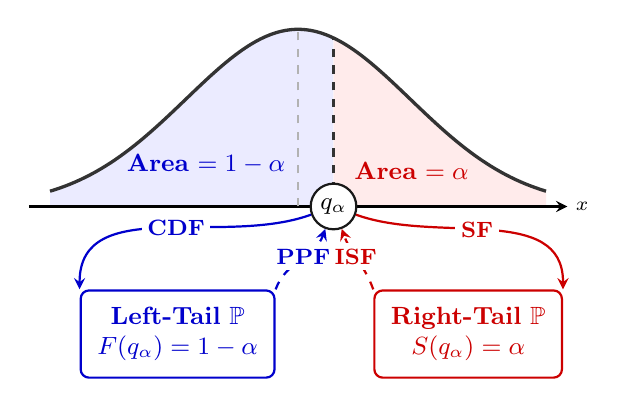
\begin{tikzpicture}[>=stealth, thick, scale=0.9]
            % Define the standard normal curve
            \def\gauss#1{2.5*exp(-0.4*0.5*(#1)^2)}
            
            % --- Shading Areas ---
            \fill[blue!8!white] (-3.5, 0) -- plot[domain=-3.5:0.5, samples=50] (\x, {\gauss{\x}}) -- (0.5, 0) -- cycle;
            \fill[red!8!white] (0.5, 0) -- plot[domain=0.5:3.5, samples=50] (\x, {\gauss{\x}}) -- (3.5, 0) -- cycle;
            
            % --- Draw Plot and Axes ---
            \draw[very thick, black!80] plot[domain=-3.5:3.5, samples=100] (\x, {\gauss{\x}});
            \draw[->, thick] (-3.8, 0) -- (3.8, 0) node[right] {$x$};
            
            % --- Markers and Labels ---
            % Mean line
            \draw[dashed, black!30] (0,0) -- (0,{\gauss{0}});
            % q_\alpha indicator line
            \draw[dashed, black!80, thick] (0.5, 0) -- (0.5, {\gauss{0.5}});
            
            % Area Text Labels
            \node[text=blue!80!black, font=\small] at (-1.3, 0.6) {\textbf{Area} $= 1-\alpha$};
            \node[text=red!80!black, font=\small] at (1.6, 0.5) {\textbf{Area} $= \alpha$};
            
            % The central q_\alpha node
            \node[circle, draw=black!90, fill=white, inner sep=2pt, font=\small, thick] (X) at (0.5, 0) {$q_\alpha$};
            
            % --- Logic Nodes (Bottom Layer) ---
            \tikzstyle{logicbox} = [rectangle, draw, thick, fill=white, rounded corners=1ex, align=center, inner sep=6pt, font=\small]
            
            \node[logicbox, draw=blue!80!black, text=blue!80!black] (P) at (-1.7, -1.8) {
                \textbf{Left-Tail} $\boldsymbol{\Pp}$ \\
                $F(q_\alpha) = 1-\alpha$
            };
            
            \node[logicbox, draw=red!80!black, text=red!80!black] (SF) at (2.4, -1.8) {
                \textbf{Right-Tail} $\boldsymbol{\Pp}$ \\
                $S(q_\alpha) = \alpha$
            };
            
            % --- Arrows ---
            \tikzstyle{arrowlabel} = [fill=white, inner sep=2pt, font=\footnotesize\bfseries]
            
            % --- Left Side (Blue) ---
            % CDF: Solid arrow pointing from x_0 to the outer edge of the Left \Pp box
            \draw[->, blue!80!black] (X) to[out=-160, in=90] node[arrowlabel, pos=0.45] {CDF} (P.north west);
            % PPF: Dashed arrow curving from the inner edge of the Left \Pp box back to x_0
            \draw[->, blue!80!black, dashed] (P.north east) to[out=70, in=-110] node[arrowlabel, pos=0.55] {PPF} (X);
            
            % --- Right Side (Red) ---
            % SF: Solid arrow pointing from x_0 to the outer edge of the Right \Pp box
            \draw[->, red!80!black] (X) to[out=-20, in=90] node[arrowlabel, pos=0.45] {SF} (SF.north east);
            % ISF: Dashed arrow curving from the inner edge of the Right \Pp box back to x_0
            \draw[->, red!80!black, dashed] (SF.north west) to[out=110, in=-70] node[arrowlabel, pos=0.55] {ISF} (X);

        \end{tikzpicture}
        }
        

        \begin{itemize}
            \item \subhdr{Expectation}: $\E[X] = \sum x p_X(x) = \int x f_X(x) dx$ .
            \item \subhdr{Expected Value Rule for Func. of RVs}: \\ $\E[g(X)] = \sum g(x) p_X(x) = \int g(x) f_X(x) dx$.
            \item \subhdr{Linearity}: $\E[aX+b] = a\E[X] + b$.
            \item \subhdr{Variance}: \\ $\Var(X) = \E[(X-\E[X])^2] = \E[X^2] - \E[X]^2$. \\ $\Var(aX+b) = a^2\Var(X)$. \\ $ \Var(\sum X_i) = \sum \Var(X_i) + 2\sum_{i<j}\Cov(X_i,X_j)$.
            \item \subhdr{Covariance}: $\Cov(X,Y) = \E[XY] - \E[X]\E[Y]$.\\ $\Cov(X,X) = \Var(X)$.
            \item \subhdr{Correlation}: Location/scale invariant: \\  $\rho(X,Y) = \dfrac{\Cov(X,Y)}{\sigma_X \sigma_Y} = \E[\dfrac{(X-\E[X])}{\sigma_X}\dfrac{(Y-\E[Y])}{\sigma_Y}]$
            \item \subhdr{Properties}: \\ $\Cov(aX,bY+Z) = ab\Cov(X,Y) + a\Cov(X,Z)$. 
            \item \subhdr{Covariance Matrix ($\Sigma$)}: $\mathbf{X} \in \R^k$: \\
            $\Sigma = \E\sqbr{(\mathbf{X}-\E[\mathbf{X}])(\mathbf{X}-\E[\mathbf{X}])^{T}}$ \\
            $\Sigma = \Var(\mathbf{X}) = \Cov(\mathbf{X}, \mathbf{X}) = "\Cov(\mathbf{X})"$
            \begin{itemize}
                \item \subhdr{$\Sigma \succeq 0$} $\iff v^\T \Sigma v \geq 0, \forall v \in \R^k$. $\lambda_i \geq 0, \forall i$
                \item \subhdr{Elements:} $\Sigma_{ij} = \Cov(X_i, X_j) $.\quad $\Sigma_{ii} = \Var(X_i)$.
                \item \subhdr{Affine Map:} $A \in \R^{m \times k}$ and $b \in \R^m$ (constant): \\
                            $\Var(A\mathbf{X} + b) = A\Var(\mathbf{X})A^\T = A\Sigma A^\T$
            \end{itemize}
        \end{itemize}

        \hdr{Transformations \& Convolutions}
        \begin{itemize}
            \item \subhdr{1D Transform (monotonic)}: $Y=g(X) \implies$ \\ $f_Y(y) = f_X(g^{-1}(y))|\frac{d}{dy}g^{-1}(y)|$. \\ $p_Y(y) = p_X(g^{-1}(y))$
            \item \subhdr{1D Transform (general)}: $Y=g(X) \implies$ \\ $f_Y(y) = d_y F_Y(y) = d_y (\Pp(g(X) \leq y))$
            \item \subhdr{2D Transform}: $f_{X,Y}(x,y) = f_{U,V}(u,v)|\det J|^{-1}$ \\ where Jacobian $J = \frac{\partial(x,y)}{\partial(u,v)}$.
            \item \subhdr{Convolutions}: For $X \indep Y$, \\ $f_{X+Y}(t) = \int_{-\infty}^\infty f_X(x)f_Y(t-x)dx$.
        \end{itemize}

        \hdr{Advanced Conditioning}
        \begin{itemize}
            \item \subhdr{Conditional $\E$ and $\Var$ as a Random Variable}: \\ $\E[X|Y]=g(Y)$, \quad $\Var(X|Y)=h(Y)$.
            \item \subhdr{Iterated Expectation}: $\E[X] = \E[\E[X|Y]]$.
            \item \subhdr{Total Var.}: $\Var(X) = \E[\Var(X|Y)] + \Var(\E[X|Y])$.
            \item \subhdr{Random Sums}: $Y = \sum_{i=1}^N X_i$, with $N$ random: \\ $\Var(Y) = \E[N]\Var(X) + \Var(N)(\E[X])^2$.
        \end{itemize}

        \section*{Bernoulli \& Poisson Processes}

        \hdr{Definitions \& Arrival Counts}
        \begin{itemize}
            \item \subhdr{Bernoulli (Discrete)}: i.i.d. trials $X_i \in \{0,1\}$. $\Pp(X_i=1)=p$. $\E[X_i]=p, \Var(X_i)=p(1-p)$.
            \item \subhdr{Poisson (Continuous)}: Indep. increments. Small $\delta$: $\Pp(1 \text{ arr})=\lambda\delta+O(\delta^2), \Pp(0)=1-\lambda\delta+O(\delta^2), \Pp(>1)=O(\delta^2)$.
            \item \subhdr{Count Distributions}:
            \begin{itemize}
                \item \textbf{Ber} ($S_n$ in $n$ slots): $S_n \sim \text{Bin}(n,p) \implies$
                \begin{itemize}
                    \item $\Pp(S_n=k)=\binom{n}{k}p^k(1-p)^{n-k}$.
                    \item $\E[S_n]=np, \Var(S_n)=np(1-p)$.
                \end{itemize}

                \item \textbf{Poi} ($N_\tau$ in time $\tau$): $N_\tau \sim \text{Pois}(\lambda\tau) \implies$
                \begin{itemize}
                    \item $\Pp(N_\tau=k)=\frac{(\lambda\tau)^k e^{-\lambda\tau}}{k!}=P(k,\tau)$.
                    \item $\E[N_\tau]=\Var(N_\tau)=\lambda\tau$.
                \end{itemize}
            \end{itemize}
            \item \subhdr{Approx.}: $\text{Bin}(n,p) \xrightarrow{n, p \to \infty, 0} \text{Pois}(\lambda=np)$.
            \item \subhdr{Hack}: $\mathrm{Pois}(\lambda_1\tau_1) + \mathrm{Pois}(\lambda_2\tau_2) \sim \mathrm{Pois}(\lambda_1\tau_1+\lambda_2\tau_2)$ \\
            $N_\tau^A \indep N_t^B \implies N_\tau^A + N_t^B \sim \mathrm{Poiss}(\lambda_A \tau + \lambda_B t)$
        \end{itemize}

        \hdr{Interarrival ($T_k$) \& $k$-th Arrival ($Y_k$) Times}
        \begin{itemize}
            \item \subhdr{Bernoulli (Discrete)}: \\
                $T_k \iid \text{Geom}(p)$ (Total trials). \\
                $Y_k \sim \text{Pascal}(k,p)$ (Total trials).
            \item \subhdr{Poisson (Continuous)}: \\
                $T_k \iid \text{Exp}(\lambda) \rightarrow \E[T_k]=1/\lambda, \Var(T_k)=1/\lambda^2$.\\
                $Y_k \sim \text{Erlang}(k, \lambda) \rightarrow \E[Y_k]=k/\lambda, \Var(Y_k)=k/\lambda^2$.
        \end{itemize}

        \hdr{Process Operations \& Properties}
        \begin{itemize}
            \item \subhdr{Memorylessness}: Both restart fresh from any fixed/causally random time. \\ For Poisson: if $T_1>t \implies T_1-t \sim \text{Exp}(\lambda)$.
            \item \subhdr{Merging Independent Processes}:
            \begin{itemize}
                \item \textbf{Ber}: $\text{Ber}(p) \oplus \text{Ber}(q) \implies \text{Ber}(p+q-pq)$. \\ 
                $\Pp(\text{arr is from process 1}) = \frac{p_1}{p_1 + p_2 - p_1 p_2} $. \\ $\Pp(\text{arr is ONLY from process 1}) = \frac{p_1(1-p_2)}{p_1 + p_2 - p_1 p_2} $.
                \item \textbf{Poi}: $\text{Pois}(\lambda_1) \oplus \text{Pois}(\lambda_2) \implies \text{Pois}(\lambda_1+\lambda_2)$. \\ $\Pp(\text{arr is from process 1}) = \frac{\lambda_1}{\lambda_1+\lambda_2}$.
            \end{itemize}
            \item \subhdr{Splitting Processes (with $\indep$ coin bias $q$)}:
            \begin{itemize}
                \item \textbf{Ber} $\implies \text{Ber}(pq)$ and $\text{Ber}(p(1-q))$. \\ \trap{Resulting Bern. streams are NOT indep.}
                \item \textbf{Poi} $\implies \text{Pois}(\lambda q)$ and $\text{Pois}(\lambda(1-q))$. \\ \ok{Resulting Poisson streams ARE indep.}
            \end{itemize}
            \item \subhdr{Min/Max (Poisson Exponentials)}: \\ For $X,Y,Z \iid \text{Exp}(\lambda) \implies \min \sim \text{Exp}(3\lambda)$. \\ $\E[\min]=\frac{1}{3\lambda}$ \quad and \quad $\E[\max]=\frac{1}{3\lambda}+\frac{1}{2\lambda}+\frac{1}{\lambda}$.
            \item \ok{Usefull trick true in general:} $\min(X,Y) + \max(X,Y) = X+Y$ 
        \end{itemize}

        \hdr{Random Incidence Paradox}
        \begin{itemize}
            \item Arriving at random $t^*$ to an ongoing Poisson process. Let $U=\text{last arrival}, V=\text{next arrival}$.
            \item Forward time $V-t^* \sim \text{Exp}(\lambda)$ \\ Backward time $t^*-U \sim \text{Exp}(\lambda)$ \\ $\implies \E[V-U]=2/\lambda$.
            \item \trap{Expected interarrival time doubles ($2/\lambda$ instead of $1/\lambda$) because sampling larger intervals is proportionally more likely based on the sampling method.}
        \end{itemize}

        \hdr{Geometric Series}

        Arbitrary start index $m$ (usually $=0$). Requires $|r| < 1$.
        \[ \sum_{k=m}^{\infty} a r^k = \frac{a r^m}{1 - r} \]


%        \hdr{Markov Chains}
%        \begin{itemize}
%            \item \subhdr{Markov Property}: \\ $\Pp(X_{n+1}=j | X_0..X_n) = \Pp(X_{n+1}=j | X_n)$.
%            \item \subhdr{States}: Recurrent (always return). Transient (may never return). Periodic (returns only in multiples of $k>1$). Aperiodic (GCD of return times is 1).
%            \item \subhdr{Transition Matrix ($Q$)}: $q_{ij} = \Pp(X_{n+1}=j | X_n=i)$. $m$-step transition is $(i,j)$ element of $Q^m$. State dist at step $n$: $\vec{p}Q^n$.
%            \item \subhdr{Stationary Dist ($\vec{s}$)}: $\vec{s}Q = \vec{s}$. Unique if chain is irreducible and aperiodic. Expected return time to state $i$ is $1/s_i$.
%            \item \subhdr{Reversibility}: $s_i q_{ij} = s_j q_{ji} \implies \vec{s}$ is stationary. \\ Random walk on undirected network $\implies \vec{s} \propto$ node degree sequence.
%        \end{itemize}

        \section*{Limit Theorems}
        \hdr{Inequalities}
        \begin{itemize}
            \item \subhdr{Markov}: $\Pp(X \geq a) \leq \E[X]/a$ for $X \geq 0$.
            \item \subhdr{Chebyshev}: $\Pp(|X-\mu| \geq c) \leq \sigma^2/c^2$.
            \item \subhdr{Cauchy-Schwarz}: $|\E[XY]| \leq \sqrt{\E[X^2]\E[Y^2]}$.\\ . \hspace{48pt} $\Cov(X,Y)^2 \leq \Var(X) \Var(Y)$.
            \item \subhdr{Jensen}: $\E[g(X)] \geq g(\E[X])$ for convex $g$. Reverse if concave.
            \item \subhdr{Hoeffding}: If $X \in [a,b]$ a.s., then for all $\varepsilon>0$:
            \[ \Pp(|\overline{X_n}-\mu|\ge \varepsilon) \le 2\exp\br{-\frac{2n\varepsilon^2}{(b-a)^2}} \]
        \end{itemize}

        \hdr{Modes of Convergence}
        \begin{itemize}
            \item \subhdr{Almost Surely}: $\Pp(\lim_{n\to\infty} T_n = T) = 1$.
            \item \subhdr{In Probability}: $\forall \varepsilon>0, \Pp(|T_n-T|\ge \varepsilon) \xrightarrow{n \to \infty} 0$.
            \item \subhdr{In Distribution}: $\E[f(T_n)] \xrightarrow{n \to \infty} \E[f(T)]$ for all continuous, bounded functions $f$.
        \end{itemize}
        $a.s. \implies \text{in prob.} \implies \text{in dist}$. \\
        In dist. implies in prob. if the limit is a constant. \\
        \subhdr{Operations}: If $T_n \to T$ and $U_n \to U$ (a.s. or prob), then $T_n+U_n \to T+U$, $T_n U_n \to TU$, and $T_n/U_n \to T/U$ (if $U \neq 0$ a.s.).

        \hdr{Limit Theorems}
        Let $X_1,\dots,X_n \iid$ with $\E[X_i]=\mu$ and $\Var(X_i)=\sigma^2$.
        \begin{itemize}
            \item \subhdr{WLLN}: $\overline{X_n} \toP \mu = \E[X_i]$.
            \item \subhdr{SLLN}: $\overline{X_n} \toas \mu = \E[X_i]$.
            \item \subhdr{CLT}: $\dfrac{\overline{X_n}-\E[X_i]}{\sqrt{\Var(\overline{X_n} )}} = \sqrt{n}\dfrac{(\overline{X_n}-\mu)}{\sigma} \toD \N(0,1) $
            \textbf{Sums}: $S_n = \sum_1^n X_i \approx \N(n\mu, n\sigma^2)$.
            \item \subhdr{Multivariate CLT}: $\sqrt{n}(\overline{X_n}-\mu) \toD \N_d(0,\Sigma)$
        \end{itemize}

        \hdr{Slutsky, CMT \& Delta Method}
        \begin{itemize}
            \item \subhdr{Slutsky's Theorem}: If $T_n \toD T$ and $U_n \toP u$ (constant):
            $T_n + U_n \toD T+u$, $T_n U_n \toD Tu$, $T_n/U_n \toD T/u$. ($u \neq 0$.)
            \item \subhdr{Continuous Mapping (CMT)}: If $f$ is continuous, $T_n \xrightarrow{a.s./\Pp/\mathcal{D}} T \implies f(T_n) \xrightarrow{a.s./\Pp/\mathcal{D}} f(T)$.
            \item \subhdr{Delta Method ($\R$)}: For $g$ contsly. difftbl. at $\theta$: \\ if $\sqrt{n}(Z_n-\theta) \toD \N(0,\sigma^2)$, then: 
            \[ \sqrt{n}(g(Z_n)-g(\theta)) \toD \N(0, [g'(\theta)]^2 \sigma^2) \]
            \item \subhdr{Delta Method ($\R^d$)}: If $\sqrt{n}(T_n-\theta) \toD \N_d(0,\Sigma)$:
            \[ \sqrt{n}(g(T_n)-g(\theta)) \toD \N(0, \nabla g(\theta)^\T \Sigma \nabla g(\theta)) \]
        \end{itemize}

        \hdr{Non trivial limits}
        If $c_1=c_1(n)$, then the next limit is not trivial:
        \[ L=\lim_{n \to \infty}\Phi(2*(c_1 - a)\sqrt{n}). \]
        For example: 
        \[ c_1 = a - \frac{b}{\sqrt{n}} \implies L = \Phi(2b). \]

%        \section*{Distributions \& Properties}
%        \hdr{Key Convolutions ($X \indep Y$)}
%        \begin{itemize}
%            \item $\mathrm{Pois}(\lambda_1) + \mathrm{Pois}(\lambda_2) \sim \mathrm{Pois}(\lambda_1+\lambda_2)$.
%            \item $\mathrm{Bin}(n_1, p) + \mathrm{Bin}(n_2, p) \sim \mathrm{Bin}(n_1+n_2, p)$.
%            \item $\mathrm{Gamma}(a_1, \lambda) + \mathrm{Gamma}(a_2, \lambda) \sim \mathrm{Gamma}(a_1+a_2, \lambda)$.
%            \item $\mathrm{NBin}(r_1, p) + \mathrm{NBin}(r_2, p) \sim \mathrm{NBin}(r_1+r_2, p)$.
%            \item $\N(\mu_1, \sigma_1^2) + \N(\mu_2, \sigma_2^2) \sim \N(\mu_1+\mu_2, \sigma_1^2+\sigma_2^2)$.
%        \end{itemize}
%
%        \hdr{Order Statistics}
%        \begin{itemize}
%            \item \subhdr{CDF}: $F_{X_{(i)}}(x) = \sum_{k=i}^n \binom{n}{k} F(x)^k(1-F(x))^{n-k}$.
%            \item \subhdr{PDF}: \\ $f_{X_{(i)}}(x) = n\binom{n-1}{i-1}F(x)^{i-1}(1-F(x))^{n-i}f(x)$.
%            \item \subhdr{Uniform Order Stat}: \\ $U_i \iid \mathrm{Unif}(0,1) \implies U_{(j)} \sim \mathrm{Beta}(j, n-j+1)$.
%        \end{itemize}
%
%        \hdr{Special Properties \& Multivariate}
%        \begin{itemize}
%            \item \subhdr{Beta-Gamma Result}: For $X \sim \mathrm{Gamma}(a,\lambda)$, $Y \sim \mathrm{Gamma}(b,\lambda) \indep \implies$ \\ $\frac{X}{X+Y} \sim \mathrm{Beta}(a,b)$ and is independent of $X+Y$.
%            \item \subhdr{$\mathrm{Mult}_k(n, \vec{p})$}: Distributes $n$ items into $k$ buckets. $\Var(X_i) = np_i(1-p_i)$. $\Cov(X_i,X_j) = -np_ip_j$.
%            \item \subhdr{Multivariate Normal (MVN)}: $\vec{X}$ is MVN if every linear combination is Normal. Subvectors are MVN. If two elements are uncorrelated, they are independent.
%        \end{itemize}

        \section*{Foundation of Inference}

        \hdr{Statistical Model}
        Pair $(E, (\Pp_\theta)_{\theta\in\Theta})$ where $E$ is the sample space.
        \begin{itemize}
            \item \subhdr{Parametric}: $\Theta \subseteq \R^d$. 
            \item \subhdr{Nonparametric}: $\Theta$ infinite dimensional. 
%            \item \subhdr{Semiparametric}: Mixed (finite $\times$ infinite).
            \item \subhdr{Identifiability}: $\theta \neq \theta' \implies \Pp_\theta \neq \Pp_{\theta'}$.
        \end{itemize}

        \hdr{Parameter Estimation}
        \begin{itemize}
            \item \subhdr{Consistency}: $\hat\theta_n \toP \theta$ (weak) or $\toas \theta$ (strong).
            \item \subhdr{Bias}: $\Bias(\hat\theta) = \E[\hat\theta] - \theta$.
            \item \subhdr{Quadratic Risk}: \\ $R(\hat\theta_n) = \E[(\hat\theta_n-\theta)^2] = \Var(\hat\theta_n) + \Bias(\hat\theta_n)^2$.
            \item \subhdr{Jensen's}: Convex $f \implies \E[f(X)] \ge f(\E[X])$. \\ Concave $g \implies \E[g(X)] \le g(\E[X])$.
        \end{itemize}

        \hdr{Confidence Intervals of level $1-\alpha$}
        Random interval $\mathcal{I}_\alpha$ not depending on $\theta$ such that: \\
        $\Pp_\theta(\mathcal{I}_\alpha \ni \theta) \ge 1-\alpha$.
%        \subhdr{Bernoulli solutions} for unknown $p$ in variance: \\ 1) Conservative bound ($p(1-p)\le 1/4$), \\ 2) Solving the quadratic equation, \\ 3) Plug-in estimator $\hat{p}$.

        \hdr{Distances and Divergences}
        \begin{itemize}
            \item \subhdr{Total Variation (TV)}: $\max_{A} |\Pp_\theta(A)-\Pp_{\theta'}(A)|$. \\
            Discrete: $\frac{1}{2}\sum |p_\theta(x)-p_{\theta'}(x)| \left( = \frac{1}{2}\int dx \right)$. \\ 
            (Metric: Symmetric, triangle inequality).
            \item \subhdr{Kullback-Leibler (KL)}: $\E_\theta[\log(p_\theta(X)/p_{\theta'}(X))]$. \\Positive, definite, but \textbf{not} sym., no triangle ineq..
        \end{itemize}

        \section*{Methods of Estimation}

        \hdr{Maximum Likelihood (MLE)} 
        $\hat\theta_n^{\text{MLE}} = \argmax_{\theta} \ell_n(\theta) = \argmax_{\theta} \ln(L_n(X_{1:n};\theta)).$
        \begin{itemize}
            \item \subhdr{Concavity}: $\ell_n$ is strictly concave $\iff \mathbb{H}\ell_n(\theta) \prec 0$.
            \item \subhdr{Fisher Information}: In 1D: $I(\theta) = -\E[\ell_1''(\theta)]$. \\ In general: $I(\theta) = -\E[\mathbb{H}\ell_1(\theta)]$.
            \item \subhdr{Asymptotics}: Under regularity conditions (interior true param, identifiable, etc.):
            \[ \sqrt{n}(\hat\theta_n^{\text{MLE}}-\theta^*) \toD \N_d(0, I(\theta^*)^{-1}) \]
        \end{itemize}
        \trap{The asymptotic Var is $I(\theta^*)^{-1}$, without $n$ scaln.}

        \hdr{Method of Moments (MM)}
        $m_k(\theta) = \E_\theta[X^k]. \quad \hat{m}_k = \frac{1}{n}\sum X_i^k$. \\
        $m_k(\hat{\theta}_n^{MM}) = \hat{m}_k, \quad \text{for } k = 1, 2, \dots, d$
        \begin{itemize}
            \item \subhdr{Asymptotics}: $\sqrt{n}(\hat\theta_n^{MM}-\theta) \toD \N(0,\Gamma(\theta))$ \\ via Delta Method (uses Jacobian of $M^{-1}$). 
        \end{itemize}
        MLE is generally more accurate, MM comput. easier.

        \hdr{M-Estimation}
        Estimate $\mu^*$ minimizing $Q(\mu) = \E[\rho(X_1,\mu)]$.
        \begin{itemize}
            \item $\rho=(x-\mu)^2 \implies \mu^*$ is the mean.
            \item $\rho=|x-\mu| \implies \mu^*$ is the median.
            \item $\rho=-\log L_1(x,\theta) \implies$ MLE.
        \end{itemize}
        \subhdr{Asymptotics}: Let $J(\mu) = \E[\nabla^2 \rho(X,\mu)]$ and \\ $K(\mu) = \Cov(\nabla \rho(X,\mu))$. Then:\\
        $\sqrt{n}(\hat\mu_n-\mu^*) \toD \N(0, J^{-1}KJ^{-1})$ \\
        (For log-likelihood MLE, $J=K=I$).

        \section*{Hypothesis Testing}

        \hdr{Testing Basics \& Master Logic}
        \begin{enumerate}
            \item State null / alternative: $H_0: \theta \in \Theta_0$ vs $H_1: \theta \in \Theta_1$.
            \item Choose statistic $T_n(X_{1:n};\theta)$.
            \item Determine distribution of $T_n$, under $H_0$:  $T_n \sim ?Z?$.
            \item Compute p-value or set rejection region $R$. \\ Test $\psi = \1_{\{R\}}$.
            \item Reject $H_0$ if p-value $\le \alpha$ (or $\psi=1$).
            \item Always state assumptions.
        \end{enumerate}
        \begin{itemize}
            \item \subhdr{Type I Error ($\alpha_\psi$)}: Reject true $H_0$. \\ Probability $\alpha_\psi(\lambda) = \Pp_\lambda(\psi = 1)$ for $\lambda \in \Theta_0$.
            \item \subhdr{Type II Error ($\beta_\psi$)}: Fail to reject false $H_0$. \\ Probability $\beta_\psi(\lambda) = \Pp_\lambda(\psi = 0)$ for $\lambda \in \Theta_1$.
            \item \subhdr{Power ($\pi_\psi$)}: $1-\beta(\theta)$ for $\theta \in \Theta_1$. Often $\inf_{\theta\in\Theta_1}(1-\beta_\psi(\theta))$.
            \item \subhdr{Test Level/Size}: $\sup_{\theta\in \Theta_0}\Pp_\theta(\psi = 1) \le \alpha$. \\ Controls worst-case Type I error probability.
            \item \subhdr{Asympt. Level}: $\lim\limits_{n \to \infty} \sup\limits_{\theta \in \Theta_0} \mathbb{P}_\theta(\psi_n = 1) \le \alpha$
            \item \subhdr{p-value}: Under $H_0$, smallest level $\alpha$ at which $H_0$ is rejected, or probability of result at least as extreme as observed.
            %\item \subhdr{Neyman--Pearson Lemma}: For simple $H_0$ vs simple $H_1$, most powerful size-$\alpha$ test rejects for large $\frac{L(\theta_1)}{L(\theta_0)}$.
            \item \subhdr{CI / Test Duality}: For many regular problems: Reject $H_0:\theta=\theta_0$ at level $\alpha \iff \theta_0 \notin (1-\alpha)\text{ CI}$.
        \end{itemize}
        \trap{Failing to reject $H_0$ does \emph{not} prove $H_0$. \\ Statistical significance $\neq$ practical significance.}

        \hdr{Power Reminders}
        Power increases with: Larger sample size $n$, larger effect size, smaller variance / noise, larger $\alpha$ (but Type I error also increases).

        \hdr{Quantiles}
        \begin{itemize}
            \item \subhdr{Quantile of order $1-\alpha$} is the number $q_\alpha$ defined by:
            \begin{itemize}
                \item Lower Tail: $\Pp(X \leq q_\alpha) = 1 - \alpha $
                \item Upper Tail: $\Pp(X > q_\alpha) = \alpha$. (Top $\alpha$.)
                \item CDF Relation: $F(q_\alpha) = 1 - \alpha \implies q_\alpha = F^{-1}(1-\alpha)$
            \end{itemize}
            \item \subhdr{Examples}: \\ $\Pp(X \leq q_{0.05}) = 0.95$, $\Pp(X \leq q_{0.7}) = 0.3$.
            \item \subhdr{Quantiles of Standard Normal ($X \sim \N(0,1)$)}
            \begin{itemize}
                \item Sym. $q_{1-\alpha} = -q_\alpha$. \quad $\Pp(|X| \leq q_{\alpha/2}) = 1 - \alpha$.
                \item $\Pp(|X| > q_{\alpha/2}) = \alpha = 2(1 - \Phi(q_{\alpha/2}))$.
                \item Common Values: $q_{0.025} = 1.96$, $q_{0.05} = 1.645$
            \end{itemize}
        \end{itemize}

        \hdr{Exam Rescue Strip}
        \begin{enumerate}
            \item Identify parameter of interest.
            \item Identify data structure: 1-sample / 2-sample / paired / count / proportion.
            \item Check assumptions: normal? indep? known $\sigma$?
            \item Choose exact vs asymptotic method.
            \item Write statistic, null distribution, rejection rule / p-value.
            \item Interpret in words, including assumptions.
        \end{enumerate}
        \trap{For two-sided tests, use both tails / absolute value logic. For one-sided tests, align rejection direction with $H_1$. Check whether variance is known, unknown, equal, or unequal before choosing $z$ / pooled $t$ / Welch.}

        \hdr{One-Sample Tests}
        \begin{itemize}
            \item \subhdr{Wald Test (1D)}: (For p-vals $\Pp=\Pp_{\theta_0}$.)
            
            \noindent\resizebox{\linewidth}{!}{
                \begin{tabular}{r|c|c|c}
                & $H_0: \theta = \theta_0$ & $H_0: \theta \le \theta_0$ & $H_0: \theta \ge \theta_0$ \\
                & $H_1: \theta \neq \theta_0$ & $H_1: \theta > \theta_0$ & $H_1: \theta < \theta_0$ \\
                \hline
                Wald test $\psi$ & $\1\{|W| > q_{\alpha/2}\}$ & $\1\{W > q_\alpha\}$ & $\1\{W < -q_\alpha\}$ \\
                p-value & $\Pp(|W| > |W^{\text{obs}}|)$ & $\Pp(W > W^{\text{obs}})$ & $\Pp(W < W^{\text{obs}})$ \\
                asymp. p-val & $\Pp(|Z| > |W^{\text{obs}}|)$ & $\Pp(Z > W^{\text{obs}})$ & $\Pp(Z < W^{\text{obs}})$ \\
                \end{tabular}
            }
            \begin{itemize}
                \item \textbf{$\sqrt{n}$ scaling}: $W_n \toD \N(0,1)$.
                \[ W_n = \frac{(\hat\theta_n-\theta_0)}{\sqrt{\widehat{\Var(\hat\theta)}}} = \sqrt{n I(\hat\theta_n)} (\hat\theta_n-\theta_0) \toD[H_0] \N(0,1) \]

                \item \textbf{$n$ scaling}: $T_n \toD \chi^2_1$. \quad Test $\psi = \1\{T_n > q_\alpha^{(\chi^2_1)}\}$:
                \[ T_n = n I(\hat\theta_n) (\hat\theta_n-\theta_0)^2 \toD \chi^2_1 \ \text{under } H_0\]
            \end{itemize}
            \trap{We dont need to use MLE, but we need consistent $(\sqrt{n})\sqrt{\widehat{\Var(\hat\theta)}}$ , and asymptotically normal $W_n$.}


            \item \subhdr{Student's T-test for $\mu$}: $X_i\iid \N(\mu,\sigma^2 (\text{unknown}))$.

            \noindent\resizebox{\linewidth}{!}{
            \begin{tabular}{r|c|c|c}
            & $H_0: \mu = \mu_0$ & $H_0: \mu \le \mu_0$ & $H_0: \mu \ge \mu_0$ \\
            & $H_1: \mu \neq \mu_0$ & $H_1: \mu > \mu_0$ & $H_1: \mu < \mu_0$ \\
            \hline
            T-Test $\psi$ & $\1\{|T| > q_{\alpha/2}^{t_{n-1}}\}$ & $\1\{T > q_\alpha^{t_{n-1}}\}$ & $\1\{T < -q_\alpha^{t_{n-1}}\}$ \\
            \end{tabular}
            }
            \vspace{2pt}
            \[ T_n = \sqrt{n}\frac{(\overline{X_n} - \mu_0)}{\sqrt{\tilde{S}_n^2}} \sim t_{n-1} \ \text{under }H_0 \]
            \trap{$\tilde{S}_n^2$ UNBIASED! $\tilde{S}_n^2 = \frac{n}{n-1}S_{pop}^2$}
            \item \subhdr{Test for variance}: $X_{i_n}\iid \N(\mu,\sigma^2 (\text{unknown}))$.
            \[ T_n=\frac{(n-1)\tilde{S}_n^2}{\sigma_0^2}\sim \chi^2_{n-1}\ \text{under }H_0 \]

            \item \subhdr{$z$-test for mean}: If $X_i\iid \N(\mu,\sigma^2)$ or large $n$ and $\sigma$ known:
            $ Z=\frac{\bar X-\mu_0}{\sigma/\sqrt n}\sim \N(0,1)\ \text{under }H_0 $
            \item \subhdr{Proportion test}: If $X\sim \mathrm{Bin}(n,p)$ and $n$ large:
            $ Z=\frac{\hat p-p_0}{\sqrt{p_0(1-p_0)/n}} \approx \N(0,1) $

        \end{itemize}

        \hdr{Two-Sample Tests}
        \begin{itemize}
            \item \subhdr{2-S. T-test}: $X_{i_n}\iid \N(\mu_x,\sigma_x^2), Y_{i_m}\iid \N(\mu_y,\sigma_y^2)$. \\
            $H_0: \mu_x -\mu_y \leq 0, \quad H_1: \mu_x -\mu_y > 0$.
            \[ T=\frac{(\overline{X_n} - \overline{Y_m}) - (\mu_x - \mu_y)}{\sqrt{S_X^2/n_X+S_Y^2/n_Y}} \sim t_N \]
            \textbf{Approx. dof} (Welch--Satterthwaite): 
            \[ N \approx \dfrac{(S_X^2/n + S_Y^2/m)^2}{\dfrac{\left(S_X^2/n\right)^2}{n-1}+\dfrac{\left(S_Y^2/m\right)^2}{m-1}} \gtrapprox \min(n,m)\]

%
%            \item \subhdr{Paired $t$}: Use differences $D_i=X_i-Y_i \sim \N$:
%            $ T=\frac{\bar D-\mu_{D,0}}{S_D/\sqrt n}\sim t_{n-1} $
%
%            \item \subhdr{Parametric Asymp Test}: $H_0: \Delta_c = \Delta_d$ vs $H_1: \Delta_d > \Delta_c$. ($n,m \to \infty$): \\
%            $ \frac{\overline{X_n} - \bar{Y}_m - (\Delta_d-\Delta_c)}{\sqrt{\hat\sigma_d^2/n + \hat\sigma_c^2/m}} \toD \N(0,1) $
%
%            \item \subhdr{Two indep means, equal var}: If $X_i\iid \N(\mu_X,\sigma^2)$, $Y_j\iid \N(\mu_Y,\sigma^2)$: \\
%            $S_p^2=\frac{(n_X-1)S_X^2+(n_Y-1)S_Y^2}{n_X+n_Y-2}$ \\
%            $ T=\frac{(\bar X-\bar Y)-\Delta_0}{S_p\sqrt{1/n_X+1/n_Y}} \sim t_{n_X+n_Y-2} $
%

        \end{itemize}

        \subhdr{Fisher's Exact Test}: $H_0: \text{Variables are } \indep$. \\Assumes $H_0$ and the marginal totals of the table are fixed.
        \vspace{-8pt}
        \begin{flushleft}
            $\begin{array}{r|cc|c}
                & B_1 & B_2 & \text{Total} \\ \hline
                A_1 & a & b & a+b \\
                A_2 & c & d & c+d \\ \hline
                \text{Total} & a+c & b+d & n
            \end{array}
            \quad
            T = \frac{\binom{a+b}{a} \binom{c+d}{c}}{\binom{n}{a+c}}$
        \end{flushleft}
        

        \hdr{Likelihood-Ratio Test (LRT)}

        $H_0: \theta \in \Theta_0$. (Fix $d-r$ params.) \\With MLEs $\hat\theta_n^\mathrm{MLE}$ (all) and $\hat\theta_n^\mathrm{MLE_C}$ (constrained):
        \[
        T_n = -2\ln \left( \frac{\sup_{\Theta_0}L_n(\theta)}{\sup_{\Theta}L_n(\theta)} \right) = -2\ln \left( \frac{L_n(\hat\theta_n^\mathrm{MLE_C})}{L_n(\hat\theta_n^\mathrm{MLE})} \right) 
        \]
        $ T_n = 2\left( \ell_n( \hat\theta_n^\mathrm{MLE} ) - \ell_n( \hat\theta_n^\mathrm{MLE_C} ) \right) \toD \chi^2_{d-r}$  \\
        $\psi = \1\{T_n > q_\alpha(\chi^2_{d-r})\}$, $\mathbf{d-r}= \dim(\Theta) - \dim(\Theta_0)$.
        \trap{We fix the complement of $\Theta_0$ ($r$ params.)}

        % \subhdr{Score Test}: Evaluate slope of log-lik at null. Asymptotically $\chi^2_1$ in scalar case: $S=\frac{U(\theta_0)^2}{I(\theta_0)}$.
        \columnbreak
        \section*{Nonparametric Tests \& GOF}

        \hdr{Goodness of Fit (Discrete / $\chi^2$)}
        Let $X_1,\dots,X_n \iid P$ on the support $\set{0,\dots,K}$. 
        \begin{itemize}
            \item $|\text{support}| = K+1$.
            \item Cell counts $N_j := \sum_{i=1}^n \1\set{X_i=j}$.  $n = \sum_{j=0}^K N_j$.
        \end{itemize}   

        \begin{itemize}
            \item \subhdr{Hypotheses \& Test Statistics}:
            \begin{itemize}
                \item \textbf{Parametric family:} \\ $H_0:\ P\in\set{\Pp_\theta}_{\theta\in\Theta\subseteq\R^d}$ vs $H_1:\ P\notin\set{\Pp_\theta}_{\theta\in\Theta\subseteq\R^d}$.
                \begin{itemize}
                    \item Fit params: $\hat\theta_0 = \hat\theta_{H_0}^{\mathrm{MLE}}$. Let $f_{\hat\theta}(j) := \Pp_{\hat\theta}(X=j)$.
                    \item $\displaystyle T_n = n\sum_{j=0}^K \frac{\br{N_j/n - f_{\hat\theta}(j)}^2}{f_{\hat\theta}(j)}  \toD[H_0] \chi^2_{K-d}$
                \end{itemize}
                \trap{For $\hat\theta$ use counts in bins, not the original $X_i$'s.}
                \item \textbf{Fixed distribution:} $H_0: \mathbf{p} = \mathbf{p}^0 \in \Delta_K$, $\hat{p}_j = N_j/n $.
                \begin{itemize}
                    \item $\displaystyle T_n = n\sum_{j=0}^K \frac{\br{\hat{p}_j - p_j^0}^2}{p_j^0}  \toD[H_0] \chi^2_{K}$
                \end{itemize}
            \end{itemize}
            
            \item \subhdr{Equivalent Form (Observed vs Expected)}:
            \begin{itemize}
                \item Observed $O_j := N_j$, Expected $E_j := n p_j$ \\ (using $p_j^0$ or $f_{\hat\theta}(j)$ depending on $H_0$).
                \item $\displaystyle T_n = \sum_{j=0}^K \frac{\br{O_j - E_j}^2}{E_j}  \toD[H_0] \chi^2_{K-d}$ 
            \end{itemize}
            
            \item \subhdr{Degrees of Freedom: $\mathbf{K-d}$}:
            \begin{itemize}
                \item Support size is $K+1$.
                \item Subtract $1$ DoF due to sum constraint $\sum N_j = n$.
                \item Subtract $d$ DoF for estimating $d$ parameters. \\(\textbf{Note:} $d=0$ for a Fixed Distribution).
                \item Total DoF $= \br{K+1} - 1 - d = K-d$.
            \end{itemize}
        \end{itemize}

        \trap{If $p_j$'s are fully known (i.e., no parameters are fitted), use:  $DoF = \br{K+1} - 1 = K$, not $K-d$. \\
        More generally, if the support has $m$ cells, use: \\ $DoF = m - 1 - d$. Always count the number of fitted parameters actually estimated from the data.}



%        \hdr{Python Hints for $\chi^2$ GOF}
%        \begin{itemize}
%            \item $(O_0,\dots,O_K)$ (counts for each cell.) = \\ \texttt{obs = np.bincount(x, minlength=K+1)}. 
%            \item Fit $\hat\theta$ under $H_0$, then \texttt{exp = n * f(theta\_hat)} ensuring \texttt{exp.sum()==n}.
%            \item \subhdr{Manual Stat}: \texttt{stat = ((obs-exp)**2/exp).sum()}
%            \item \subhdr{Manual df}: \texttt{df = K-d}
%            \item \subhdr{Manual p-val}: \\ \texttt{pval = 1 - scipy.stats.chi2.cdf(stat, df)}
%            \item \subhdr{SciPy Shortcut}: \\ \texttt{scipy.stats.chisquare(obs, f\_exp=exp, ddof=d)}. \\ (Default df in SciPy is $(K+1)-1=K$. Passing \texttt{ddof=d} adjusts it to $K-d$).
%        \end{itemize}
%        \trap{If cell probs $p_j$ are fully known (no fitted params), $\text{df} =(K+1)-1=K$, not $K-d$. If support has $m$ cells, use $\text{df} =m-1-d$. Always count fitted parameters actually estimated from the data. In code, \texttt{chisquare(..., ddof=d)} is only correct if $d$ params were fitted from the same data used in the test.}


        \hdr{Goodness of Fit (Continuous / CDF)}
        \textbf{Empirical CDF}: $F_n(t) = \frac{1}{n}\sum \1\{X_i \le t\}$. \\
        \textbf{Glivenko-Cantelli}: $\sup_t |F_n(t)-F(t)| \toas 0$. \\
        \textbf{Donsker's}: $\sqrt{n}\sup_t |F_n(t)-F(t)| \toD \sup_t |B(t)|$. \\

        \subhdr{Kolmogorov-Smirnov (KS) Test}: \textbf{Pivotal} for any sample size $n$, provided: The null distribution is continuous. The null distribution is fully specified.
        \[ \text{Test: } \psi = \1\{T_n > q_\alpha^\text{KS}\} \]
        \[ T_n = \sup_{t\in\R} \sqrt{n}|F_n(t)-F^0(t)| \sim\]
        Let $X_{(1)}\leq X_{(2)}\leq\dots\leq X_{(n)}$ be the reordered sample.\\ The expression for $T_n$ reduces to:
        \[T_n = \sqrt{n}\max_{1\le i\le n}\max\left(D_i^-, D_i^+\right)\]
        \[D_i^- = \left|\frac{i-1}{n}-F^0\left(X_{(i)}\right)\right|, D_i^+ = \left|\frac{i}{n}-F^0\left(X_{(i)}\right)\right|\]

        \subhdr{Kolmogorov-Lilliefors (KL) Test}: \\ Tests Gaussianity where params ($\hat\mu, \hat\sigma^2$) are estimated. \textit{Donsker} is invalid; uses different quantiles.
        \[ \text{Test: } \psi = \1\{T_n > q_\alpha^\text{KL}\} \]
        \[ T_n = \sup_{t\in\R}\left|F_n(t)-\Phi_{\hat{\mu},\hat{\sigma}^2}(t)\right| \]
        where $\hat{\mu}=\overline{X}_n$, $\hat{\sigma}^2=S_n^2$.

%        \subhdr{Cram\'er-Von Mises}: $d^2 = \int [F_n(t)-F(t)]^2 dF(t)$.
%        \subhdr{Anderson-Darling}: Integrand divided by $F(t)(1-F(t))$ to increase sensitivity to the tails.

        \hdr{Q-Q Plots}
        Plot $(F^{-1}(i/n), F_n^{-1}(i/n))$ against $y=x$. Visually checks if distributions match.

        \begin{center}
        \setlength{\tabcolsep}{1pt}
        \renewcommand{\arraystretch}{0.2}
        \begin{tabular}{cc}
        \scriptsize Heavy tails & \scriptsize Right skewed \\
        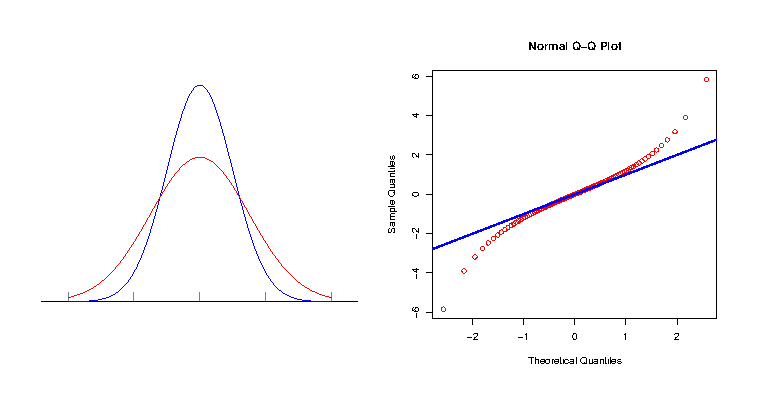
\includegraphics[width=0.48\columnwidth,trim={1cm 0 0 1cm},clip]{figures/1.pdf} &
        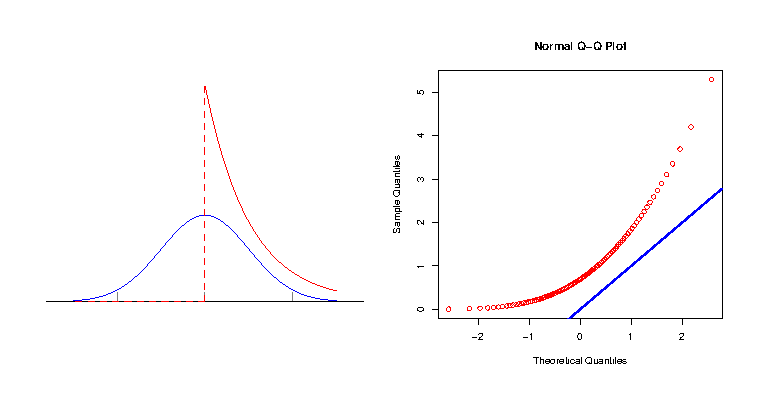
\includegraphics[width=0.48\columnwidth,trim={1cm 0 0 1cm},clip]{figures/2.pdf} \\
        \scriptsize Left skewed & \scriptsize Light tails \\
        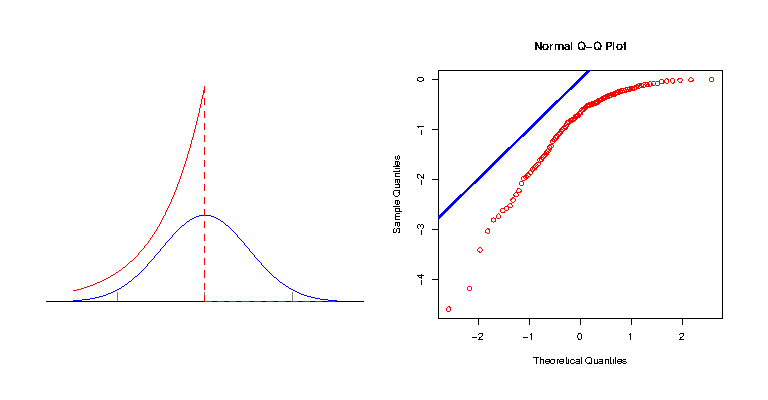
\includegraphics[width=0.48\columnwidth,trim={1cm 0 0 1cm},clip]{figures/3.pdf} &
        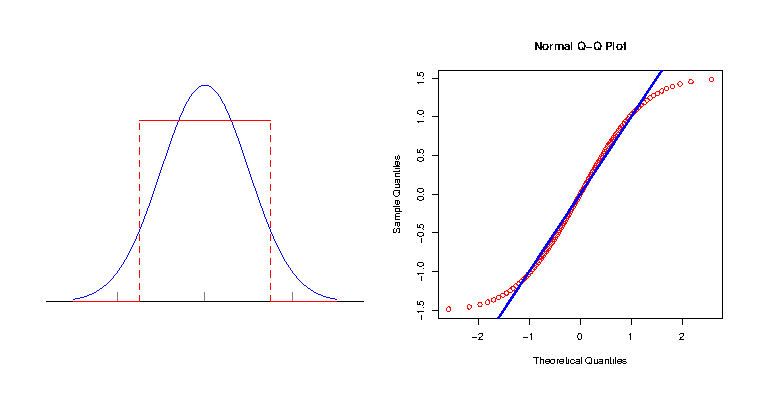
\includegraphics[width=0.48\columnwidth,trim={1cm 0 0 1cm},clip]{figures/4.pdf} \\
        \end{tabular}
        \end{center}
        \vspace{-10pt}
        Horiz. = Theoretical quantiles. Vert. = Sample quant.\\
        
        
        \columnbreak


        \section*{Multiple Testing}


        \subhdr{FWER: Family-Wise Error Rate}\\
        \hdr{Bonferroni Method (FWER)}
        Controls \textbf{FWER}: ($\leq \alpha$.)
        \begin{itemize}
            \item \subhdr{Rule}: Reject the $i$-th test $\iff P_i \leq \alpha/N$.
            \item \subhdr{Proof}: $\text{FWER} = \Pp_{\mu_i=0} \Big( \bigcup_{i=1}^N \{P_i < \frac{\alpha}{N}\} \Big)$ \\ $\text{FWER} \le \sum_{i=1}^N \Pp_{\mu_i=0}(|T_i| > q_{\frac{\alpha}{2N}}) = N \cdot \frac{\alpha}{N} = \alpha$.
        \end{itemize}
        \trap{Often way too conservative, leading to low power (no discoveries).}
        
        \hdr{Holm-Bonferroni Method (FWER)}
        Controls \textbf{FWER}: ($\leq \alpha$.)
        \begin{itemize}
            \item \subhdr{Ordering}: Order p-values: $P_{(1)} \le P_{(2)} \le \dots \le P_{(N)}$.
            \item \subhdr{Rule}: Reject $H_{(i)}$ if $P_{(j)} \le \frac{\alpha}{N-j+1}$ for all $j \le i$. 
            \\ (Step-down: Stop at the first $i$ where $P_{(i)} > \frac{\alpha}{N-i+1}$ and fail to reject all subsequent hypotheses).
        \end{itemize}
        \ok{Uniformly more powerful than the standard Bonferroni method.}

        \subhdr{FDR: False Discovery Rate} \\
        \hdr{Benjamini-Hochberg Method (FDR)}
        Controls \textbf{FDR}: ($\leq \alpha$.)
        \begin{itemize}
            \item \subhdr{Ordering}: Order p-values: $P_{(1)} \le P_{(2)} \le \dots \le P_{(N)}$.
            \item \subhdr{Rule}: Let $i_{\max} := \max\left\{i : P_{(i)} < i \cdot \frac{\alpha}{N}\right\}$. Reject all tests $(i)$ such that $i \le i_{\max}$.
        \end{itemize}
        \ok{Intuitively rejects tests with the smallest p-values and is less conservative than (Holm-)Bonferroni.}
        

        \section*{Bayesian Statistics \& Inference}
        
        
        \hdr{Basics, Priors and Posteriors}
        \begin{itemize}
            \item \subhdr{Universal Bayes}: \[\Pr(\theta|x) = \frac{\Pr(\theta)\Pr(x|\theta)}{\Pr(x)}\]
            \textbf{Notation:} $Pr = f (=p)$, $f$ if cont. ($p$ if disc.). \\
            $\Pr(x) = \sum_{\Theta} \Pr(\theta')\Pr(x|\theta') \left( = \int_{\Theta} d\theta' \right)$
  
            \item \subhdr{Bayesian Setup}: Prior $\pi(\theta)$. (or $p_\Theta(\theta)$, or $f_\Theta(\theta)$).\\ Likelihood $L_n(X_{1:n}|\theta)$. (or $p_{X|\Theta}(x|\theta)$, $f_{X|\Theta}(x|\theta)$).
            \item \subhdr{Bayes' Formula / Posterior}: \\ $\pi(\theta|X_{1:n}) = \pi_{\Theta|X_{1:n}}(\theta|x_{1:n})$ 
                            \[\pi(\theta|X_{1:n}) = \dfrac{\pi(\theta)L_n(X_{1:n}|\theta)}{L_n(X_{1:n})} \propto \pi(\theta)L_n(X_{1:n}|\theta).\]
                            Marginal $L_n(X_{1:n}) =  \int_\Theta \pi(\theta)L_n(X_{1:n}|\theta) d\theta$.
        \end{itemize}
        \trap{Deterministic Priors dont change given any data.}
        \hdr{Bayesian Estimators}
        \begin{itemize}
            \item \subhdr{Posterior Mean/LMS}: $\hat\theta^{(\pi)} = \hat{\theta}_{\text{LMS}} = \E[\Theta|X_{1:n}]$ \\ 
            $\hat\theta^{\pi} = \int_\Theta \theta \pi(\theta|X_{1:n})d\theta = \argmin_{\hat{\theta}}\E[(\Theta-\hat{\theta})^2|X_{1:n}]$.
            \item \subhdr{MAP}: $\hat{\theta}_{\text{MAP}} = \argmax_\theta \pi(\theta|X_{1:n})$.
            \item \subhdr{LLMS}: \\ $\hat{\Theta}_{LLMS} = \E[\Theta] + \frac{\Cov(\Theta,X)}{\Var(X)}(X-\E[X])$.
            %\item \subhdr{Posterior Predictive}: \\ $p(x_{\text{new}}|x)=\int p(x_{\text{new}}|\theta)\pi(\theta|x)\,d\theta$.
            \item \subhdr{Confidence Region of level $\alpha$}: \\ deterministic subset $\mathcal{R}$ such that $\Pp(\theta\in\mathcal{R}|X_{1:n}) = 1-\alpha$. Depends on prior choice.
        \end{itemize}

        \hdr{Conjugate Priors}
        \begin{itemize}
            \item \subhdr{Bernoulli-Beta}: if $p \sim \text{Beta}(a,b), \hspace{1pt} X_i|p \sim \text{Bern}(p)$. \\
            $ \implies p|X_{1:n} \sim \text{Beta}(a+\sum X_i, b+n-\sum X_i)$. \\ 
            Prior pdf: $\pi(p) \propto p^{a-1}(1-p)^{b-1}$. \\
            Likelihood: $L_n \propto p^{\sum X_i}(1-p)^{n-\sum X_i}$. \\
            $\pi(p|X_{1:n}) \propto p^{(a+\sum X_i)-1}(1-p)^{(b+n-\sum X_i)-1}$. 
            \item \subhdr{Poiss-Gamma}: $\Lambda \sim \text{Gam}(\alpha, \lambda), X_i|\Lambda \sim \text{Poiss}(\Lambda)$. \\ $\implies \Lambda|X_{1:n} \sim \text{Gamma}(\alpha + \sum X_i, \lambda + n)$
            \item \subhdr{Normal-Normal}: Normal mean + Normal prior.\\ $\implies$ posterior Normal.
        \end{itemize}

        \hdr{Non-informative \& Jeffreys Priors}
        \begin{itemize}
            \item \subhdr{Improper prior}: $\int \pi(\theta)d\theta = \infty$ (e.g., $\propto 1$). \\ \ok{Can still yield a proper posterior.}
            \item \subhdr{Jeffreys Prior}: $\pi_J(\theta) \propto \sqrt{\det I(\theta)}$. if $ \eta = \phi(\theta)$:
            \[ \pi_J(\phi^{-1}(\eta))\left|\frac{1}{\phi'(\phi^{-1}(\eta))}\right| = \tilde{\pi}_J(\eta) \propto \sqrt{\det \tilde{I}(\eta)}.\]
            \\ i.e., satisfies \textbf{reparameterization invariance}.
            \begin{itemize}
                \item $X \sim \text{Bern}(p) \implies \pi_J(p) \propto p^{-1/2}(1-p)^{-1/2}$.
                \item $X \sim \N(\mu, \sigma^2 (\text{known})) \implies \pi_J(\mu) \propto 1$.
            \end{itemize} 
        \end{itemize}
        
        \columnbreak
\section*{Linear Regression}

\hdr{Modeling Assumptions}
Describe $\Pp$ partially via regression function: $f(x) = \E[Y|X=x]$.
Theoretical min of $\E[(Y-a-bX)^2]$ gives:
$b^* = \Cov(X,Y)/\Var(X)$, $a^* = \E[Y]-b^*\E[X]$. \\
\subhdr{Noise}: $\varepsilon = Y - (a^*+b^*X)$. $\E[\varepsilon]=0$, $\Cov(X,\varepsilon)=0$. \\
\subhdr{1D LSE}: 
\[ \hat{b} = \frac{\overline{XY}-\bar{X}\bar{Y}}{\overline{X^2}-\bar{X}^2}, \quad \hat{a} = \bar{Y} - \hat{b}\bar{X} \]

\hdr{Multivariate LSE}
Matrix Form: $\mathbf{Y} = \X\beta^* + \boldsymbol{\varepsilon}$. Assuming $\rank(\X)=p$:
\[ \hat{\boldsymbol{\beta}} = \argmin_\beta \Norm{\mathbf{Y}-\X\beta}_2^2 = (\X^\T\X)^{-1}\X^\T\mathbf{Y} \]
\subhdr{Geometric}: $\X\hat{\boldsymbol{\beta}}$ is the orthogonal projection of $\mathbf{Y}$ onto the column space of $\X$. \\ Projection matrix: $P = \X(\X^\T\X)^{-1}\X^\T$.

\hdr{Statistical Inference for LSE}
Assume $\X$ deterministic, homoscedastic ($\varepsilon_i \iid$), Gaussian noise $\boldsymbol{\varepsilon} \sim \N_n(0,\sigma^2 I_n)$.
\begin{itemize}
    \item \subhdr{Distribution}: $\hat{\beta} \sim \N_p(\beta^*, \sigma^2(\X^\T \X)^{-1})$.
    \item \subhdr{Risk}: $\E[\Norm{\hat{\beta}-\beta^*}_2^2] = \sigma^2 \tr((\X^\T \X)^{-1})$.
    \item \subhdr{Prediction Error}: $\E[\Norm{\mathbf{Y}-\X\hat{\beta}}_2^2] = \sigma^2(n-p)$.
    \item \subhdr{Unbiased Variance}: $\hat\sigma^2_{unb} = \frac{1}{n-p}\Norm{\mathbf{Y}-\X\hat{\beta}}_2^2$ (with residuals $\hat{\boldsymbol{\varepsilon}} = \mathbf{Y} - \X\hat{\beta}$).
\end{itemize}

\hdr{Hypothesis Testing Framework \& Contrasts}
Evaluate linear combinations via a contrast vector $u \in \R^p$.
\begin{itemize}
    \item \subhdr{Example:} $u = [1, -1, 0, \dots, 0]^\T$ isolates $\beta_1$ and $\beta_2$ to test if $\beta_1 \le \beta_2$.
    \item \subhdr{Hypotheses:} $H_0: u^\T \beta^* \le 0 \quad \text{vs} \quad H_1: u^\T \beta^* > 0$.
\end{itemize}

\subhdr{1. Pivotal Quantity Construction}
The test statistic is built from independent Normal and $\chi^2$ components:
\begin{itemize}
    \item \textbf{Numerator (Normal)}: The normalized estimator:
    \[ Z = \frac{u^\T \hat{\beta} - u^\T \beta^*}{\sigma \sqrt{u^\T (\X^\T \X)^{-1} u}} \sim \N(0,1) \]
    \item \textbf{Denominator (Chi-Squared)}: The variance ratio:
    \[ V = \frac{\hat{\sigma}^2_{unb}}{\sigma^2} \sim \frac{\chi^2_{n-p}}{n-p} \]
    \item \textbf{Student's t Pivot}: Because $\hat{\sigma}^2_{unb} \indep \hat{\beta}$, the unknown true variance $\sigma^2$ cancels out when taking $Z / \sqrt{V}$:
    \[ \frac{u^\T \hat{\beta} - u^\T \beta^*}{\hat{\sigma}_{unb} \sqrt{u^\T (\X^\T \X)^{-1} u}} \sim t_{n-p} \]
\end{itemize}

\subhdr{2. Execution Recipe}
\begin{enumerate}
    \item \textbf{Fit Model}: Calculate $\hat{\beta}$, residuals $\hat{\boldsymbol{\varepsilon}}$, and $\hat{\sigma}^2_{unb}$.
    \item \textbf{Standard Error}: Compute the specific error for the contrast: 
    \[ \se(u^\T \hat{\beta}) = \hat{\sigma}_{unb}\sqrt{u^\T(\X^\T \X)^{-1}u} \]
    \item \textbf{Test Statistic ($T_n$)}: Evaluate under the strict boundary condition of the null hypothesis ($u^\T \beta^* = 0$):
    \[ T_n = \frac{u^\T \hat{\beta}}{\se(u^\T \hat{\beta})} \]
    \item \textbf{Decision Rule}: Find the critical threshold $s = q_{1-\alpha}(t_{n-p})$. Reject $H_0$ if $T_n > s$.
\end{enumerate}

\trap{Type I Error Control: If the true parameter is strictly interior ($u^\T\beta^* < 0$), the actual probability of falsely rejecting $H_0$ is strictly bounded below $\alpha$. The threshold $s$ guarantees exact $\alpha$-level control right at the boundary.}

\hdr{Variable Significance Tests}
\begin{itemize}
    \item \subhdr{Single Variable}: $H_0: \beta_j=0$. Let $\gamma_j = [(\X^\T \X)^{-1}]_{jj}$. The test statistic is:
    \[ T_n^{(j)} = \frac{\hat\beta_j}{\sqrt{\hat\sigma^2_{unb}\gamma_j}} \sim t_{n-p} \]
    Reject if $|T_n^{(j)}| > q_{\alpha/2}(t_{n-p})$.
    \item \subhdr{Bonferroni Correction}: Test a group of variables $S$. Reject if any $|T_n^{(j)}| > q_{\alpha/(2k)}$ where $k=|S|$.
\end{itemize}
\ 

%        \section*{Generalized Linear Model (GLM)}
%
%        \hdr{Exponential Family}
%        $k$-param: $f_\theta(y) = \exp[\sum_{i=1}^k \eta_i(\theta)T_i(y) - B(\theta)]h(y)$. \\
%        \subhdr{1-param Canonical form}: 
%        \[ f_\theta(y) = \exp\br{\frac{y\theta-b(\theta)}{\phi}+c(y,\phi)} \]
%        $\theta$ is canonical parameter. $\phi$ is dispersion parameter.
%        \begin{itemize}
%            \item \subhdr{Moments}: $\E[Y] = b'(\theta)$ and $\Var(Y) = b''(\theta)\phi$.
%        \end{itemize}
%
%        \hdr{GLM Architecture}
%        Generalizes linear regression via:
%        \begin{enumerate}
%            \item \textbf{Random component}: $Y|X \sim$ exponential family.
%            \item \textbf{Predictor}: $\eta = X^\T \beta$.
%            \item \textbf{Link function}: $g(\mu) = X^\T \beta$, where $\mu = \E[Y|X]$. \\
%            Requires $g$ to be monotone increasing and differentiable.
%        \end{enumerate}
%
%        \hdr{Canonical Link}
%        Links mean $\mu$ directly to canonical parameter $\theta$: $g(\mu) = \theta$. 
%        Since $\mu = b'(\theta)$, the canonical link is $g(\mu) = (b')^{-1}(\mu)$. 
%        If $\phi>0$, canonical link is strictly increasing. \\
%        \subhdr{Bernoulli Example}: 
%        $\theta = \log(\frac{p}{1-p})$ and $b(\theta) = \log(1+e^\theta)$. 
%        Canonical link is \textbf{logit}: $\theta = \log(\frac{\mu}{1-\mu}) = X^\T \beta$.
%
%        \hdr{Log-Likelihood}
%        $\theta_i = h(X_i^\T \beta)$ where $h = (b')^{-1} \circ g^{-1}$.
%        If the canonical link is used, $h$ is the identity: $\theta_i = X_i^\T \beta$.
%        \[ \ell_n(\mathbf{Y},\mathbb{X},\beta) = \sum_i \frac{Y_i X_i^\T \beta - b(X_i^\T \beta)}{\phi} + \text{const} \]
%        Using the canonical link ensures $\ell(\theta)$ is \textbf{strictly concave} (guaranteeing a unique MLE). Other links may yield local maxima.
        \columnbreak

        \section*{Data Analysis}
        \hdr{Causality}
        \subhdr{The fundamental problem of causal inference}: \\
        We can never observe the \textbf{counterfactual}. It is impossible to simultaneously observe both the treated and untreated outcomes for the same subject.

        \hdr{Randomized Control Trials (RCTs)}
        Important: \textbf{Consent} is important, correctly \textbf{informing} the participants. \\
        We can try to identify \textbf{confounder} variables before randomizing, \textbf{stratify}, and \textbf{randomize} within each group. Then aggregate results.
        \begin{itemize}
            \item \textbf{Randomized}: Causality problem, neutralizing both known and unknown confounding variables.
            \item \textbf{Controlled}: Involves at least one control group (comparative counterfactual).
            \item \textbf{Trial}: A study design where researchers administer a treatment and track outcomes moving forward.
            \item \textbf{Double-Blind}: Participants \& researchers don't know who is in which group till end. (placebo effect, confirmation or observer bias).
        \end{itemize}
        
        \underline{\subhdr{Confounders}}
        If we are trying to identify the relation between $X$ and $Y$. A confounder is a variable $Z$ that affects both variables or is affected by an underlying cause $U$ that affects both variables. 
        Making $X$ and $Y$ correlated without having a causal relation between them. \\
        \trap{Assuming a reversed causality because of a confounder. Example below:}

%       \begin{itemize}
%            \item $D$: Decision to consent (or not) to the study.
%            \item $X$: Actual participation / Trial group assignment (Exposure, resulting from D).
%            \item $Y$: Polio incidence rate after the study is finished (Outcome, affected by C).
%            \item $U$: Socioeconomic Status (SES - unmeasured root cause of both C and D).
%            \item $C$: Living Environment / Hygiene Level (proxy confounder, caused by U and causes Y).
%        \end{itemize}

        \vspace{-10pt}
        
        \begin{flushleft}

            \begin{tikzcd}[row sep=small, column sep=small]

            & |[label=above:{\text{Source of Confounding}}]| Z \arrow[dl, "\text{(proxy-of) Cause}"'] \arrow[dr, "\text{(proxy-of) Cause}"] & \\

            X \arrow[rr, leftrightarrow, dashed, "\text{correlation}"'] & & Y

            \end{tikzcd}

        \end{flushleft}



        \underline{\subhdr{p-values}}: If we run a poorly designed experiment to get data to regress $Y$ on $\mathbf{X}$, 
        even with a lot of data, getting small p-value for some components of $\mathbf{X}$ indicated a valid correlation, \textbf{not causation}. 
        Could be used as a \textit{first approach} to identify possible causal \textbf{theories/mechanism}, necessary for \textbf{scientific} claims.

        \begin{itemize}
            \item \textbf{Metric of Incompatibility:} A p-value indicates the degree of incompatibility between observed data and a specified statistical model constructed under a set of assumptions, along with a “null hypothesis”.
            \item \textbf{Misinterpretation of Probability:} It does \textit{not} measure the probability that a studied hypothesis is true or that the data were produced by random chance alone.
            \item \textbf{Threshold Limitations:} Scientific, business, and policy decisions should not rely solely on whether a p-value crosses a specific threshold (e.g., $p < 0.05$). P-values supplement, but do not replace, scientific reasoning.
            \item \textbf{Integrity through Transparency:} Proper inference requires full reporting. Selective reporting (\textit{p-hacking}) renders conclusions unreliable, whereas transparency regarding all tests conducted minimizes bias.
            \item \textbf{Independence from Magnitude:} Statistical significance does not measure effect size or the importance of a result. Separate estimation methods, such as confidence intervals or Bayesian approaches, should be used to quantify uncertainty and effect magnitude.
        \end{itemize}


 %       \begin{itemize}
 %           \item P-values can indicate how incompatible the data are with a specified statistical model.
 %           \item P-values do not measure the probability that the studied hypothesis is true, or the probability that the data were produced by random chance alone.
 %           \item Scientific conclusions and business or policy decisions should not be based only on whether a p-value passes a specific threshold.
 %           \item Proper inference requires full reporting and transparency.
 %           \item A p-value, or statistical significance, does not measure the size of an effect or the importance of a result.
 %           \item By itself, a p-value does not provide a good measure of evidence regarding a model or hypothesis.
 %           
%
 %           \item \textbf{P-values shouldn't replace scientific reasoning}. It provides some support towards rejecting the null hypothesis.
%
 %           \item Scientific conclusion, funding, decision making \textbf{should not solely depend on p-values}.
%
 %           \item P-value is a \textbf{description of data}, in relation to model assumption, statistical model and hypotheses.
%
 %           \item If the scientific practice involves \textbf{p-hacking}, which is testing many hypotheses but only reporting the significant ones, then scientific conclusions become \textbf{less reliable}.
%
 %           \item By being \textbf{transparent} about the scientific reasoning and tests conducted, p-values do not pose extra bias in scientific discovery.
%
 %           \item P-values are \textbf{independent from the size of the effect}. There are other statistical approaches that can address the size of an effect and its associated uncertainty (e.g., estimation methods like intervals or Bayesian approaches).
%
%
 %       \end{itemize}
 %       
        \subhdr{Notes}: Individual $\neq$ Aggregate. Is the variable measured a good proxy for variable of interest?


        \hdr{W. Most Pub. Research Find. is False}
        \begin{itemize}
            \item \subhdr{$R$ (Pre-study Odds):} Ratio of true relationships to no relationships.
            \item \subhdr{$u$ (Bias):} Prop. of analyses reported as findings due to manipulation/selective reporting.
            \item \subhdr{$n$ (Teams):} Number of independent research teams testing the same hypothesis.
            \item \subhdr{Positive Predictive Value (PPV)} The post-study probability that a statistically significant finding is actually true: $PPV = \frac{\text{True Positives}}{\text{Total Positive Findings}}$
        \end{itemize}

        \textbf{The Six Corollaries}
        Research findings are \textit{less} likely to be true when:
        \begin{enumerate}
            \item \subhdr{Small Studies:} $\downarrow$ sample sizes yield $\downarrow$ statistical power ($1-\beta$).
            \item \subhdr{Small Effect Sizes:} Postulated effects are barely distinguishable from noise.
            \item \subhdr{Massive Testing:} High-throughput testing of thousands of hypotheses shrinks $R$.
            \item \subhdr{High Flexibility:} Broad freedom in study design, definitions, and analytical modes.
            \item \subhdr{Interest \& Prejudice:} Financial/personal conflicts artificially inflate bias ($u$).
            \item \subhdr{``Hot'' Fields:} $\uparrow$ independent teams ($n$) competing for impressive results $\to \uparrow$ false positives.
        \end{enumerate}

%\subhdr{Standard Model (No Bias):}
%$$PPV = \frac{(1 - \beta)R}{(1 - \beta)R + \alpha}$$
%
%\subhdr{Model with Bias ($u$):}
%$$PPV = \frac{(1 - \beta)R + u\beta R}{R + \alpha - \beta R + u - u\alpha + u\beta R}$$
%
%\subhdr{Model with Multiple Teams ($n$):}
%$$PPV = \frac{R(1 - \beta^n)}{R + 1 - (1 - \alpha)^n - R\beta^n}$$
%
%\hdr{Practical Benchmarks}
%\begin{tabular}{@{}l@{\hspace{4pt}}l@{\hspace{4pt}}c@{\hspace{4pt}}l@{}}
%\toprule
%\textbf{Study Design} & \textbf{$R$} & \textbf{$u$} & \textbf{PPV} \\ \midrule
%Powered RCT & 1:1 & 0.10 & 0.85 \\
%Conf. Meta-analysis & 2:1 & 0.30 & 0.85 \\
%Exploratory Epi. & 1:10 & 0.30 & 0.12--0.20 \\
%Discovery Research & 1:1000 & 0.80 & 0.0010 \\ \bottomrule
%\end{tabular}

%        \section*{Matrix Algebra: Inverses \& Regression}
%
%        \hdr{1. The Golden Rule of "Cancellation"}
%        \begin{itemize}
%            \item \subhdr{Standard Algebra}: $ax = ay \implies x = y$.
%            \item \subhdr{Matrix Algebra}: $AX = AY \not\hspace{-4pt}\implies X = Y$.
%            \item \subhdr{Rule}: Matrix $A$ can only be cancelled by multiplying by $A^{-1}$.
%            \item If $A$ is \subhdr{square \& invertible}: $X = Y$ is guaranteed.
%            \item If $A$ is \subhdr{singular/rectangular}: Cannot cancel. $X$ and $Y$ can differ entirely but map to the same output space.
%        \end{itemize}
%
%        \hdr{2. Anatomy \& Invertibility}
%        A matrix requires two properties for a true, two-sided inverse: it must be \subhdr{square} and have \subhdr{full rank} (linearly independent rows/cols).
%
%        \vspace{2pt}
%        \begin{tabular}{@{}ll>{\raggedright\arraybackslash}p{2.2cm}@{}}
%        \toprule
%        \subhdr{Shape} & \subhdr{Rank Limit} & \subhdr{Inverse Type} \\
%        \midrule
%        Square ($n \times n$) & Full ($n$) & \textbf{True}: $A^{-1}$ \\
%        Tall ($n > p$) & Col Rank ($p$) & \textbf{Left}: $L \implies LA = I$ \\
%        Wide ($p < n$) & Row Rank ($p$) & \textbf{Right}: $R \implies AR = I$ \\
%        \bottomrule
%        \end{tabular}
%        \vspace{2pt}
%
%        \hdr{3. Left vs. Right: The "Squish"}
%        \begin{itemize}
%            \item \subhdr{Tall Matrices} (e.g., Design $\mathbf{X}$): Map smaller space $\to$ larger space. No info lost $\implies$ \subhdr{Left inverse} exists ($\mathbf{L X} = \mathbf{I}$).
%            \item \subhdr{Wide Matrices} (e.g., Transposed $\mathbf{X}^\T$): Map larger space $\to$ smaller space. Info is compressed ("squished"). Cannot un-squish data $\implies$ \subhdr{No left inverse}.
%        \end{itemize}
%
%        \hdr{4. Regression / Posterior Hack}
%        When solving for OLS estimator or posterior mean $\mu$, you encounter:
%        $$ \mathbf{X}^\T \mathbf{X} \mu = \mathbf{X}^\T \mathbf{Y} $$
%
%        \trap{Attempting to cancel $\mathbf{X}^\T$ directly. $\mathbf{X}^\T$ is a short/wide matrix without a left inverse!}
%
%        \subhdr{The Solution:}
%        \begin{enumerate}
%            \item Multiply tall $\mathbf{X}$ and wide $\mathbf{X}^\T$ to form block $(\mathbf{X}^\T \mathbf{X})$.
%            \item Result is a $p \times p$ \subhdr{square matrix}.
%            \item Assuming no perfect collinearity, it has a \subhdr{true inverse}: $(\mathbf{X}^\T \mathbf{X})^{-1}$.
%            \item \subhdr{Left-multiply} the entire block:
%        \end{enumerate}
%        $$ (\mathbf{X}^\T \mathbf{X})^{-1} (\mathbf{X}^\T \mathbf{X}) \mu = (\mathbf{X}^\T \mathbf{X})^{-1} \mathbf{X}^\T \mathbf{Y} $$
%        $$ \mu = (\mathbf{X}^\T \mathbf{X})^{-1} \mathbf{X}^\T \mathbf{Y} $$

    \end{multicols*}


\newpage

% =========================================================
% Final page: Distributions table
% =========================================================
\begin{table}[htpb]
    \noindent\textbf{Assumption:} We consider an i.i.d. sample $X_1, \dots, X_n$ from the specified distribution, where $\overline{X_n} = \frac{1}{n}\sum_{i=1}^n X_i$ denotes the sample mean. \\
    \textit{*Note: For the Binomial and Hypergeometric distributions, the traditional parameter $n$ (number of trials/draws) has been renamed to $m$ to avoid confusion with the sample size $n$.}
    \vspace{0.75em}

    \noindent\resizebox{\linewidth}{!}{%
    \renewcommand{\arraystretch}{1.8}
    \begin{tabular}{@{}m{0.16\linewidth}m{0.26\linewidth}m{0.08\linewidth}m{0.14\linewidth}m{0.14\linewidth}m{0.15\linewidth}m{0.12\linewidth}@{}}
    \textbf{Distribution} & \textbf{PMF/PDF \& support} & \textbf{$\E[X]$} & \textbf{$\Var(X)$} & \textbf{MLE $\hat{\theta}$} & \textbf{$\mathcal{I}(\theta)$} & \textbf{Asymp. Var. $V$} \newline $(\Var(\hat{\theta}) \approx V/n)$ \\
    \hline
    Bernoulli \newline $\mathrm{Bern}(p)$ \newline $p \in [0,1]$ \newline \scriptsize\textit{Indicator of success.}
    & $\Pp(X=k)=p^k(1-p)^{1-k}$ \newline $k\in\{0,1\}$
    & $p$ & $p(1-p)$
    & $\overline{X_n}$
    & $\dfrac{1}{p(1-p)}$
    & $p(1-p)$
    \\ \hline
    Binomial \newline $\mathrm{Bin}(m,p)$ \newline $m \in \mathbb{Z}^+,\ p \in [0,1]$ \newline \scriptsize\textit{Successes in $m$ indep. trials.}
    & $\Pp(X=k)=\binom{m}{k}p^k(1-p)^{m-k}$ \newline $k\in\{0,1,\dots,m\}$
    & $mp$ & $mp(1-p)$
    & $\dfrac{\overline{X_n}}{m}$ \newline (if $m$ known)
    & $\dfrac{m}{p(1-p)}$
    & $\dfrac{p(1-p)}{m}$
    \\ \hline
    Geometric (Total Failures) \newline $\mathrm{Geom}(p)$ \newline $p \in [0,1]$ \newline \scriptsize\textit{Failures before 1st success.}
    & $\Pp(X=k)=(1-p)^k p$ \newline $k\in\{0,1,2,\dots\}$
    & $\dfrac{1-p}{p}$ & $\dfrac{1-p}{p^2}$
    & $\dfrac{1}{1+\overline{X_n}}$
    & $\dfrac{1}{p^2(1-p)}$
    & $p^2(1-p)$
    \\ \hline
    Geometric (Total Trials) \newline $\mathrm{Geom}(p)$ \newline $p \in [0,1]$ \newline \scriptsize\textit{Trials until 1st success.}
    & $\Pp(X=t)=(1-p)^{t-1} p$ \newline $t\in\{1,2,\dots\}$
    & $\dfrac{1}{p}$ & $\dfrac{1-p}{p^2}$
    & $\dfrac{1}{\overline{X_n}}$
    & $\dfrac{1}{p^2(1-p)}$
    & $p^2(1-p)$
    \\ \hline
    Neg.Binomial / Pascal \newline (Total Failures $r$) \newline $\mathrm{NBin}(k,p)$ ($k$ arrivals)\newline $k \in \mathbb{Z}^+,\ p \in [0,1]$ \newline \scriptsize\textit{Failures before $k$th success.}
    & $\Pp(X=r)=\binom{r+k-1}{k-1}p^k(1-p)^r$ \newline $r\in\{0,1,2,\dots\}$
    & $\dfrac{k(1-p)}{p}$ & $\dfrac{k(1-p)}{p^2}$
    & $\dfrac{k}{k+\overline{X_n}}$ \newline (if $k$ known)
    & $\dfrac{k}{p^2(1-p)}$
    & $\dfrac{p^2(1-p)}{k}$
    \\ \hline
    Neg.Binomial / Pascal \newline (Total Trials $t$) \newline $\mathrm{Pascal}(k,p)$ ($k$ arrivals)\newline $k \in \mathbb{Z}^+,\ p \in [0,1]$ \newline \scriptsize\textit{Trials until $k$th success.}
    & $\Pp(X=t) = \binom{t-1}{k-1} p^k (1-p)^{t-k}$ \newline $t\in\{k, k+1, \dots\}$
    & $\dfrac{k}{p}$ & $\dfrac{k(1-p)}{p^2}$
    & $\dfrac{k}{\overline{X_n}}$ \newline (if $k$ known)
    & $\dfrac{k}{p^2(1-p)}$
    & $\dfrac{p^2(1-p)}{k}$
    \\ \hline
    Poisson \newline $\mathrm{Pois}(\lambda)$ \newline $\lambda > 0$ \newline \scriptsize\textit{Rare events.}
    & $\Pp(X=k)=e^{-\lambda}\dfrac{\lambda^k}{k!}$ \newline $k\in\{0,1,2,\dots\}$
    & $\lambda$ & $\lambda$
    & $\overline{X_n}$
    & $\dfrac{1}{\lambda}$
    & $\lambda$
    \\ \hline \hline
    Uniform \newline $\mathrm{Unif}(a,b)$ \newline $a < b$
    & $f(x)=\dfrac{1}{b-a}$ \newline $x\in[a,b]$
    & $\dfrac{a+b}{2}$ & $\dfrac{(b-a)^2}{12}$
    & $\hat{a}=X_{(1)}$ (biased) \newline $\hat{b}=X_{(n)}$ (biased)
    & N/A
    & $\mathcal{O}(1/n^2)$
    \\ \hline
    Normal \newline $\mathcal N(\mu,\sigma^2)$ \newline $\mu \in \mathbb{R},\ \sigma^2 > 0$ \newline \scriptsize\textit{Standardizes to $\mathcal{N}(0,1)$}
    & $f(x)=\dfrac{1}{\sigma\sqrt{2\pi}}e^{-(x-\mu)^2/(2\sigma^2)}$ \newline $x\in\mathbb R$ \newline $\E[(X-\mu)^p]=\sigma^p(p-1)$ for $p$ even ($=0$ ow.)
    & $\mu$ & $\sigma^2$
    & $\hat{\mu}=\overline{X_n}$ \newline $\hat{\sigma}^2=S^2_{\text{pop}}$ (biased)
    & $\mathrm{diag}\Big(\dfrac{1}{\sigma^2}, \dfrac{1}{2\sigma^4}\Big)$
    & $\mathrm{diag}(\sigma^2, 2\sigma^4)$
    \\ \hline
    Multiv. Normal \newline $\mathcal N(\boldsymbol{\mu},\boldsymbol{\Sigma})$ \newline $\boldsymbol{\mu} \in \mathbb{R}^d,\ \boldsymbol{\Sigma} \succ 0$
    & $f(\mathbf{x})=\dfrac{1}{\sqrt{(2\pi)^d|\boldsymbol{\Sigma}|}} e^{-\frac{1}{2}(\mathbf{x}-\boldsymbol{\mu})^\T\boldsymbol{\Sigma}^{-1}(\mathbf{x}-\boldsymbol{\mu})}$ \newline $\mathbf{x}\in\mathbb R^d$
    & $\boldsymbol{\mu}$ & $\boldsymbol{\Sigma}$
    & $\hat{\boldsymbol{\mu}}=\overline{\mathbf{X}_n}$ \newline $\hat{\boldsymbol{\Sigma}}=\frac{1}{n}\sum_{i=1}^n (\mathbf{X}_i \!-\! \hat{\boldsymbol{\mu}})$ \newline $\quad \times (\mathbf{X}_i \!-\! \hat{\boldsymbol{\mu}})^\T$
    & Block matrix \newline involving $\boldsymbol{\Sigma}^{-1}$
    & $\mathcal{I}(\boldsymbol{\mu},\boldsymbol{\Sigma})^{-1}$
    \\ \hline
    Exponential \newline $\mathrm{Expo}(\lambda)$ \newline $\lambda > 0$ \newline \scriptsize\textit{Memoryless:} \newline \textit{$\Pp(X_{>s+t}|X_{>s}) = \Pp(X_{>t})$}
    & $f(x)=\lambda e^{-\lambda x}$ \newline $x\in[0,\infty)$
    & $\dfrac{1}{\lambda}$ & $\dfrac{1}{\lambda^2}$
    & $\dfrac{1}{\overline{X_n}}$
    & $\dfrac{1}{\lambda^2}$
    & $\lambda^2$
    \\ \hline
    Gamma (Rate) / Erlang \newline $\mathrm{Gamma}(a,\lambda)$ \newline $a > 0,\ \lambda > 0$ \newline  Erlang($a = k \in \mathbb{Z}^+$) \newline ($k$ arrivals, $\Gamma(k)=(k-1)!$) \newline \scriptsize\textit{Sum of $a$ iid $\mathrm{Expo}(\lambda)$.}
    & $f(x)=\dfrac{\lambda^a}{\Gamma(a)}x^{a-1}e^{-\lambda x}$ \newline $x\in(0,\infty)$
    & $\dfrac{a}{\lambda}$ & $\dfrac{a}{\lambda^2}$
    & $\hat{a}$: No closed form \newline $\hat{\lambda}=\hat{a}/\overline{X_n}$
    & $\begin{pmatrix} \psi'(a) & -\frac{1}{\lambda} \\ -\frac{1}{\lambda} & \frac{a}{\lambda^2} \end{pmatrix}$
    & $\mathcal{I}(a,\lambda)^{-1}$
    \\ \hline
    Gamma (Scale) \newline $\mathrm{Gamma}(k,\theta)$ \newline $k > 0,\ \theta > 0$
    & $f(x)=\dfrac{1}{\theta^k\Gamma(k)}x^{k-1}e^{-x/\theta}$ \newline $x\in(0,\infty)$
    & $k\theta$ & $k\theta^2$
    & $\hat{k}$: No closed form \newline $\hat{\theta}=\overline{X_n}/\hat{k}$
    & $\begin{pmatrix} \psi'(k) & \frac{1}{\theta} \\ \frac{1}{\theta} & \frac{k}{\theta^2} \end{pmatrix}$
    & $\mathcal{I}(k,\theta)^{-1}$
    \\ \hline
    Inverse Gamma \newline $\mathrm{InvGamma}(\alpha,\beta)$ \newline $\alpha > 0,\ \beta > 0$
    & $f(x)=\dfrac{\beta^\alpha}{\Gamma(\alpha)}x^{-\alpha-1}e^{-\beta/x}$ \newline $x\in(0,\infty)$
    & $\dfrac{\beta}{\alpha-1}$ & $\dfrac{\beta^2}{(\alpha-1)^2(\alpha-2)}$ \newline ($\alpha>2$)
    & $\hat{\alpha}$: No closed form \newline $\hat{\beta}=\dfrac{\hat{\alpha}}{\frac{1}{n}\sum X_i^{-1}}$
    & $\begin{pmatrix} \psi'(\alpha) & -\frac{1}{\beta} \\ -\frac{1}{\beta} & \frac{\alpha}{\beta^2} \end{pmatrix}$
    & $\mathcal{I}(\alpha,\beta)^{-1}$
    \\ \hline
    Beta \newline $\mathrm{Beta}(a,b)$ \newline $a > 0,\ b > 0$ \newline \scriptsize\textit{Conj. prior of Binomial.}
    & $f(x)=\dfrac{\Gamma(a+b)}{\Gamma(a)\Gamma(b)}x^{a-1}(1-x)^{b-1}$ \newline $x\in(0,1)$
    & $\dfrac{a}{a+b}$ & $\dfrac{ab}{(a+b)^2(a+b+1)}$
    & $\hat{a}, \hat{b}$: No closed form
    & Matrix of \newline polygammas
    & $\mathcal{I}(a,b)^{-1}$
    \\ \hline
    Chi-Square \newline $\chi^2_\nu$ \newline $\nu \in \mathbb{Z}^+$ \newline \scriptsize\textit{Sum of $\nu$ iid $\mathcal{N}(0,1)^2$.} \newline \textit{$\chi^2_\nu \sim \mathrm{Gamma}(\nu/2, 1/2)$}
    & $f(x)=\dfrac{1}{2^{\nu/2}\Gamma(\nu/2)}x^{\nu/2-1}e^{-x/2}$ \newline $x\in(0,\infty)$
    & $\nu$ & $2\nu$
    & $\hat{\nu}$: No closed form
    & $\dfrac{\psi'(\nu/2)}{4}$
    & $\dfrac{4}{\psi'(\nu/2)}$
    \\ \hline
    Student-$t$ \newline $t_\nu$ \newline $\nu > 0$
    & $f(x)=\dfrac{\Gamma((\nu+1)/2)}{\sqrt{\nu\pi}\Gamma(\nu/2)}\Big(1+\dfrac{x^2}{\nu}\Big)^{-(\nu+1)/2}$ \newline $x\in\mathbb R$
    & $0\ (\nu>1)$ & $\dfrac{\nu}{\nu-2}\ (\nu>2)$
    & $\hat{\nu}$: No closed form
    & Complex fn \newline of $\nu$
    & $\mathcal{I}(\nu)^{-1}$
    \\ \hline \hline \hline
    Hypergeometric \newline $\mathrm{HGeom}(w,b,m)$ \newline $w,b \in \mathbb{Z}_{\ge 0}$ \newline $m \in \{1,\dots,w+b\}$ \newline \scriptsize\textit{Successes in $m$ draws without replacement.}
    & $\Pp(X=k)=\dfrac{\binom{w}{k}\binom{b}{m-k}}{\binom{w+b}{m}}$ \newline $k\in\{\dots\}$
    & $\dfrac{mw}{w+b}$ & $\dfrac{mw}{w+b}\big(1-\dfrac{w}{w+b}\big)$ \newline $\times\dfrac{w+b-m}{w+b-1}$
    & N/A
    & N/A
    & N/A
    \\ \hline \hline
    Log-Normal \newline $\mathcal{LN}(\mu,\sigma^2)$ \newline $\mu \in \mathbb{R},\ \sigma^2 > 0$
    & $f(x)=\dfrac{1}{x\sigma\sqrt{2\pi}}e^{-(\log x-\mu)^2/(2\sigma^2)}$ \newline $x\in(0,\infty)$
    & $e^{\mu+\sigma^2/2}$ & $e^{2\mu+\sigma^2}(e^{\sigma^2}-1)$
    & $\hat{\mu}=\overline{\ln X_n}$ \newline $\hat{\sigma}^2=S^2_{\ln X_n}$
    & $\mathrm{diag}\Big(\dfrac{1}{\sigma^2}, \dfrac{1}{2\sigma^4}\Big)$
    & $\mathrm{diag}(\sigma^2, 2\sigma^4)$
    \\ \hline
    \end{tabular}%
    }

    \vspace{0.75em}
    \noindent\small\textbf{Notes and Notation:}\\
    $\bullet$ $\psi'(x) = \frac{d^2}{dx^2} \ln \Gamma(x)$ is the \textbf{trigamma function}, the derivative of the digamma function.\\
    $\bullet$ $X_{(1)}$ and $X_{(n)}$ denote the sample minimum and sample maximum (order statistics) of the $n$ observations.\\
    $\bullet$ $S^2_{\text{pop}} = \frac{1}{n}\sum_{i=1}^n (X_i - \overline{X_n})^2$ is the uncorrected (biased) sample variance, representing the MLE for $\sigma^2$.\\
    $\bullet$ $S^2_{\ln X_n} = \frac{1}{n}\sum_{i=1}^n (\ln X_i - \overline{\ln X_n})^2$ is the uncorrected sample variance of the log-transformed data.\\
    $\bullet$ $\mathcal{I}(\theta)$ is the Fisher Information evaluated for a \textit{single} observation.\\
    $\bullet$ The \textbf{Asymptotic Variance} ($V$) refers to the variance of the limiting distribution: $\sqrt{n}(\hat{\theta}_n - \theta) \xrightarrow{d} \mathcal{N}(0, V)$, where $V = \mathcal{I}(\theta)^{-1}$. i.e.: $\Var(\hat{\theta}_n) \approx \frac{V}{n}$.
\end{table}

\end{document}